\chapter{ผลการดำเนินงาน}

การดำเนินงานของโปรเจคนี้จะแบ่งออกมาเป็นทั้งหมด 3 ส่วน โดยส่วนแรกคือส่วนของการจัดเก็บข้อมูลเข้าสู่ระบบโดยนำรูปภาพได้ที่ได้รับมาผ่านกระบวนการการเตรียมข้อมูลรูปภาพ 
ก่อนจะนำไปผ่านกระบวนการ OCR และการเตรียมข้อมูลตัวอักษร ก่อนจะถูกเก็บข้อมูลในระบบ ส่วนที่สองการค้นหาข้อมูล เป็นการค้นหาแบบ IR (Information retrieval) 
ที่จะนำไปโมเดล Word2Vec เข้ามาช่วยในการค้นหาคำที่มีความสัมพันธ์ใกล้เคียงกับคำค้นหา และนำคะแนน TF-IDF มาใช้เป็นคะแนนในการค้นหา และส่วนสุดท้ายคือส่วนของการทำแพลตฟอร์มเว็ปไซต์
ซึ่งในการประเมินผลการดำเนินงานนั้นเราจะทำการประเมินในส่วนแรก โดยการประเมินความถูกต้องของการทำ OCR จะมีเจ้าหน้าที่บรรณารักษ์กำหนดเกณฑ์ไว้ 
ซึ่งเกณฑ์ที่กำหนดในส่วนของความถูกต้องในการทำ OCR อยู่ที่ 75 \% และความแม่นยำในการค้นหาอยู่ที่ 75 \%

\section{ผลลัพธ์ที่ได้จากการแปลงข้อมูลรูปภาพให้เป็นข้อมูลดิจิทัล}

\subsection{ผลลัพธ์ที่ได้จากประสิทธิภาพของการหมุน}
ผลลัพธ์จากการหมุนภาพตัวอักษรทั้ง 978 ภาพ มีความคลาดเคลื่อนทั้งหมด 7.98\% ที่ยังไม่สามารถหมุนภาพให้ตรงดังภาพที่ \ref{fig:rotateErrror} 
และทำให้บางภาพแย่ลง เนื่องจากว่าบรรทัดตัวอักษรอาจจะมีสระที่ไม่สามารถทำกร่อนให้กลายเป็นเส้นบรรทัดได้

\begin{figure}[H]
    \centering
    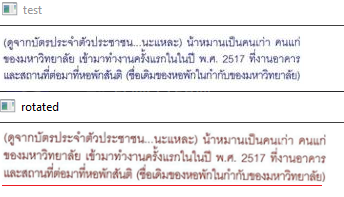
\includegraphics[scale=1]{rotateErrror}
    \caption{ภาพแสดงผลลัพธ์การหมุนรูปที่ผิดพลาด}\label{fig:rotateErrror}
\end{figure}

\subsection{ผลการเปรียบเทียบประสิทธิภาพในการทำ OCR ของ การทำการเตรียมข้อมูลรูปภาพ แต่ละแบบ}

จากการทดสอบประสิทธิภาพของการทำการเตรียมข้อมูลรูปภาพทั้งสองแบบ พบว่า 
การทำการเตรียมข้อมูลรูปภาพ แบบแรกนั้นมีจำนวนคำผิดน้อยกว่า แต่มีจำนวนคำที่ไม่สามารถแปลงเป็นดิจิทัลมากถึง 
32.71\% ดังตารางที่ \ref{tbl:imagep1} ซึ่งต่างจากการทำการเตรียมข้อมูลรูปภาพ แบบที่ 2 ที่มีค่าความถูกต้องของคำ 
74.74 \% ดังตาราง \ref{tbl:imagep2}

\subsubsection{แบบที่ 1 การใช้การคัดเลือกข้อมูล,การหมุน,การลบรูปภาพ,การลบเส้น และการจัดกลุ่ม}
\begin{table}[H]
    \caption{ตารางประเมินการทำการเตรียมข้อมูลรูปภาพแบบที่ 1 }\label{tbl:imagep1}
    \begin{tabular}{|c|c|c|p{0.1\linewidth}|p{0.1\linewidth}|c|p{0.1\linewidth}|p{0.1\linewidth}|}
        \hline
        หนังสือ                             & หน้า  & จำนวนคำทั้งหมด & จำนวนคำผิดที่ตรวจพบ & เปอร์เซ็นต์คำผิดที่ตรวจพบ(\%)    & จำนวนคำเกิน & จำนวนคำที่ไม่สามารถแปลงเป็นดิจิทัล & เปอร์เซ็นต์คำที่ไม่สามารถแปลงเป็นดิจิทัล(\%)    \\ \hline
        \multirow{2}{*}{กตเวทิตาปี 2542}      & 15    & 4         & \multicolumn{1}{c|}{4  }         & \multicolumn{1}{c|}{100 \%  } & \multicolumn{1}{c|}{0  }    & \multicolumn{1}{c|}{0  }             & \multicolumn{1}{c|}{0 \%    }\\ \cline{2-8} 
                                            & 29    & 252       & \multicolumn{1}{c|}{14 }         & \multicolumn{1}{c|}{5.56 \% }  &\multicolumn{1}{c|}{46}     &\multicolumn{1}{c|}{2 }              &\multicolumn{1}{c|}{0.79 \%} \\ \hline
        \multirow{2}{*}{กตเวทิตาปี 2556}      & 15    & 242       & \multicolumn{1}{c|}{33 }         & \multicolumn{1}{c|}{13.64 \%}  &\multicolumn{1}{c|}{2 }     &\multicolumn{1}{c|}{1 }              &\multicolumn{1}{c|}{0.41 \%} \\ \cline{2-8} 
                                            & 29    & 257       & \multicolumn{1}{c|}{20 }         & \multicolumn{1}{c|}{7.78 \% } & \multicolumn{1}{c|}{3  }    & \multicolumn{1}{c|}{10 }             & \multicolumn{1}{c|}{3.89 \% }\\ \hline
        \multirow{2}{*}{รายงานประจำปี 2544}   & 15    & 47        & \multicolumn{1}{c|}{3  }         & \multicolumn{1}{c|}{6.38 \% } & \multicolumn{1}{c|}{2  }    & \multicolumn{1}{c|}{34 }             & \multicolumn{1}{c|}{72.34 \%} \\ \cline{2-8} 
                                            & 29    & 585       & \multicolumn{1}{c|}{39 }         & \multicolumn{1}{c|}{6.67 \% } & \multicolumn{1}{c|}{3  }    & \multicolumn{1}{c|}{308}             & \multicolumn{1}{c|}{52.65 \%} \\ \hline
        \multirow{2}{*}{รายงานประจำปี 2553}   & 15    & 68        & \multicolumn{1}{c|}{0  }         & \multicolumn{1}{c|}{0 \%    } & \multicolumn{1}{c|}{0  }    & \multicolumn{1}{c|}{68 }             & \multicolumn{1}{c|}{100 \%  }\\ \cline{2-8} 
                                            & 29    & 596       & \multicolumn{1}{c|}{17 }         & \multicolumn{1}{c|}{2.85 \% } & \multicolumn{1}{c|}{8  }    & \multicolumn{1}{c|}{340}             & \multicolumn{1}{c|}{57.05 \%} \\ \hline
        \multirow{2}{*}{รายงานประจำปี 2549}   & 15    & 155       & \multicolumn{1}{c|}{53 }         & \multicolumn{1}{c|}{34.19 \%}  &\multicolumn{1}{c|}{42}     &\multicolumn{1}{c|}{45}              &\multicolumn{1}{c|}{29.03 \%} \\ \cline{2-8} 
                                            & 29    & 304       & \multicolumn{1}{c|}{22 }         & \multicolumn{1}{c|}{7.24 \% } & \multicolumn{1}{c|}{20 }    & \multicolumn{1}{c|}{13 }             & \multicolumn{1}{c|}{4.28 \%}\\ \hline
        \multicolumn{1}{|l|}{}              & total & 2510      & \multicolumn{1}{c|}{205}         & \multicolumn{1}{c|}{8.17 \% } & \multicolumn{1}{c|}{126}    & \multicolumn{1}{c|}{821}             & \multicolumn{1}{c|}{32.71 \%} \\ \hline
        \end{tabular}
        \end{table}

\subsubsection{แบบที่ 2 ใช้การลบพื้นหลัง}

\begin{table}[H]
    \caption{ตารางประเมินการทำการเตรียมข้อมูลรูปภาพแบบที่ 2}\label{tbl:imagep2}
    \begin{tabular}{|c|c|c|p{0.1\linewidth}|p{0.1\linewidth}|c|p{0.1\linewidth}|p{0.1\linewidth}|}
            \hline
            หนังสือ                             & หน้า                       & จำนวนคำทั้งหมด & จำนวนคำผิดที่ตรวจพบ & เปอร์เซ็นต์คำผิดที่ตรวจพบ(\%)    & จำนวนคำเกิน & จำนวนคำที่ไม่สามารถแปลงเป็นดิจิทัล & เปอร์เซ็นต์คำที่ไม่สามารถแปลงเป็นดิจิทัล(\%)    \\ \hline
            \multirow{2}{*}{กตเวทิตาปี 2542}      & 15                         & \multicolumn{1}{c|}{4   }      & \multicolumn{1}{c|}{4  }         & \multicolumn{1}{c|}{100\%  } & \multicolumn{1}{c|}{0 }     & \multicolumn{1}{c|}{0  }             & \multicolumn{1}{c|}{0\%    } \\ \cline{2-8} 
                                                & 29                         & \multicolumn{1}{c|}{252 }      & \multicolumn{1}{c|}{30 }         & \multicolumn{1}{c|}{11.9\% } & \multicolumn{1}{c|}{6 }     & \multicolumn{1}{c|}{9  }             & \multicolumn{1}{c|}{3.57\% } \\ \hline
            \multirow{2}{*}{กตเวทิตาปี 2556}      & 15                         & \multicolumn{1}{c|}{242 }      & \multicolumn{1}{c|}{42 }         & \multicolumn{1}{c|}{17.36\%} & \multicolumn{1}{c|}{2 }     & \multicolumn{1}{c|}{48 }             & \multicolumn{1}{c|}{19.83\%} \\ \cline{2-8} 
                                                & 29                         & \multicolumn{1}{c|}{257 }      & \multicolumn{1}{c|}{54 }         & \multicolumn{1}{c|}{21.01\%} & \multicolumn{1}{c|}{2 }     & \multicolumn{1}{c|}{62 }             & \multicolumn{1}{c|}{24.12\%} \\ \hline
            \multirow{2}{*}{รายงานประจำปี 2544}   & 15                         & \multicolumn{1}{c|}{47  }      & \multicolumn{1}{c|}{27 }         & \multicolumn{1}{c|}{57.45\%} & \multicolumn{1}{c|}{5 }     & \multicolumn{1}{c|}{5  }             & \multicolumn{1}{c|}{10.64\%} \\ \cline{2-8} 
                                                & 29                         & \multicolumn{1}{c|}{585 }      & \multicolumn{1}{c|}{101}         & \multicolumn{1}{c|}{17.26\%} & \multicolumn{1}{c|}{23}     & \multicolumn{1}{c|}{0  }             & \multicolumn{1}{c|}{0\%    } \\ \hline
            \multirow{2}{*}{รายงานประจำปี 2553}   & 15                         & \multicolumn{1}{c|}{68  }      & \multicolumn{1}{c|}{30 }         & \multicolumn{1}{c|}{44.12\%} & \multicolumn{1}{c|}{7 }     & \multicolumn{1}{c|}{0  }             & \multicolumn{1}{c|}{0\%    } \\ \cline{2-8} 
                                                & 29                         & \multicolumn{1}{c|}{596 }      & \multicolumn{1}{c|}{85 }         & \multicolumn{1}{c|}{14.26\%} & \multicolumn{1}{c|}{30}     & \multicolumn{1}{c|}{0  }             & \multicolumn{1}{c|}{0\%    } \\ \hline
            \multirow{2}{*}{รายงานประจำปี 2549}   & 15                         & \multicolumn{1}{c|}{155 }      & \multicolumn{1}{c|}{57 }         & \multicolumn{1}{c|}{36.77\%} & \multicolumn{1}{c|}{14}     & \multicolumn{1}{c|}{4  }             & \multicolumn{1}{c|}{2.58\% } \\ \cline{2-8} 
                                                & 29                         & \multicolumn{1}{c|}{304 }      & \multicolumn{1}{c|}{76 }         & \multicolumn{1}{c|}{25\%   } & \multicolumn{1}{c|}{7 }     & \multicolumn{1}{c|}{0  }             & \multicolumn{1}{c|}{0\%    } \\ \hline
            \multicolumn{1}{|l|}{}              & \multicolumn{1}{c|}{total} & \multicolumn{1}{c|}{2510}      & \multicolumn{1}{c|}{506}         & \multicolumn{1}{c|}{20.16\%} & \multicolumn{1}{c|}{96}     & \multicolumn{1}{c|}{128}             & \multicolumn{1}{c|}{5.1\%  } \\ \hline
            \end{tabular}
            \end{table}
ซึ่งจำนวนคำต่างๆในตารางนั้นถูกบันทึกและตรวจพบด้วยคน ส่วนจำนวนคำเกินนั้นจะเป็นคำที่คาดว่าเกิดจากกาอ่านพยัญชนะแยกกับสระผิด หรือบางทีมีการอ่านบรรทัดเดิมมาซ้ำทำให้มีตัวอักษร หรือคำอื่นๆที่ไม่มีอยู่ในรูปเกินออกมา
ส่วนจำนวนคำที่ไม่สามารถแปลงเป็นดิจิทัลได้นั้นจะเป็นคำที่มีอยู่ในรูปภาพแต่ไม่ผ่านการแปลงเป็นรูปแบบดิจิทัล เนื่องจาก OCR ไม่สามารถแปลงรูปหรือคำออกมาเป็นตัวหนังสือได้ หรือเกิดจากการทำ image processing 
หรือการเตรียมข้อมูลรูปภาพส่งผลให้มีคำบางคำหายไป
จากผลลัพธ์ตารางที่ \ref{tbl:imagep1} และ \ref{tbl:imagep2} ทำให้ผู้จัดทำเลือกการทำ image processing แบบที่ 2 มาใช้ในการเตรียมรูปภาพก่อนนำไป OCR
ถึงแม้ว่าจะมีจำนวนคำผิดมากกว่าในแบบที่ 1 แต่จำนวนคำที่ไม่ถูกอ่านในการทำ image processing แบบที่ 1 มีมากถึง 32.71 \% ซึ่งจะทำให้ผู้ใช้งานจะมีภาระในการตรวจสอบคำมากกว่าแบบที่ 2 

\subsection{ผลการเปรียบเทียบข้อมูล training set 2 ชุดสำหรับการทำ OCR}

โดยตอนที่เลือกข้อมูลที่ใช้การทำ OCR ทางผู้จัดได้พบว่ามีชุดข้อมูลที่ทาง Tesseract ได้ปล่อยออกมาในเว็บไซต์หลักซึ่งเป็นชุด training set ในปี 2016 เป็นชุดที่ 1
และมีข้อมูลชุด training set ที่ได้มีการอ้างอิงมาว่าเป็นชุดข้อมูลที่ดีที่สุดในปี 2019 ที่ได้รับการประเมินจาก Google เป็นชุดที่ 2
ซึ่งทำให้ผู้จัดทำนำชุดข้อมูล training set ทั้งสองชุดนี้มาทำการเปรียบเทียบว่าชุดไหนมีประสิทธิภาพมากกว่ากัน
จากการเปรียบข้อมูลทั้งสองชุดระหว่าง ชุดข้อมูลปี 2016 (ชุดที่ 1)ดังตารางที่ \ref{tbl:bigdata} ชุดข้อมูลปี 2019 (ชุดที่ 2) ดังตารางที่ \ref{tbl:smalldata} กับ
พบว่าประสิทธิภาพของข้อมูลชุดที่ 1 มีความถูกต้องอยู่ที่ 76.61 \% ซึ่งมีจำนวนคำผิดสูงกว่าประมาณ 2\% ความถูกต้องอยู่ที่ 
เมื่อเทียบกับข้อมูลชุดที่ 2 ที่มีความถูกต้องอยู่ที่ 77.41 \% แต่ว่ามีจำนวนคำเกินที่ต่างกันเป็นเท่าตัว 
และมีจำนวนคำที่ไม่สามารถแปลงเป็นดิจิทัลมากกว่า 28 คำ

\begin{table}[H]
    \caption{ตารางประเมินข้อมูลชุด training set ที่ 1}\label{tbl:bigdata}
    \begin{tabular}{|c|c|c|p{0.1\linewidth}|p{0.1\linewidth}|c|p{0.1\linewidth}|p{0.1\linewidth}|}
            \hline
            หนังสือ                             & หน้า  & จำนวนคำทั้งหมด & จำนวนคำผิดที่ตรวจพบ & เปอร์เซ็นต์คำผิดที่ตรวจพบ(\%)    & จำนวนคำเกิน & จำนวนคำที่ไม่สามารถแปลงเป็นดิจิทัล & เปอร์เซ็นต์คำที่ไม่สามารถแปลงเป็นดิจิทัล(\%)    \\ \hline
            \multirow{2}{*}{กตเวทิตาปี 2542}      & 15    & 4         & \multicolumn{1}{c|}{2  }         & \multicolumn{1}{c|}{50\%   } & \multicolumn{1}{c|}{0 }     & \multicolumn{1}{c|}{2  }             & \multicolumn{1}{c|}{50\%   } \\ \cline{2-8} 
                                                & 29    & 252       & \multicolumn{1}{c|}{34 }         & \multicolumn{1}{c|}{13.49\%} & \multicolumn{1}{c|}{12}     & \multicolumn{1}{c|}{4  }             & \multicolumn{1}{c|}{1.59\% } \\ \hline
            \multirow{2}{*}{กตเวทิตาปี 2556}      & 15    & 242       & \multicolumn{1}{c|}{37 }         & \multicolumn{1}{c|}{15.29\%} & \multicolumn{1}{c|}{0 }     & \multicolumn{1}{c|}{49 }             & \multicolumn{1}{c|}{20.25\%} \\ \cline{2-8} 
                                                & 29    & 257       & \multicolumn{1}{c|}{47 }         & \multicolumn{1}{c|}{18.29\%} & \multicolumn{1}{c|}{2 }     & \multicolumn{1}{c|}{45 }             & \multicolumn{1}{c|}{17.51\%} \\ \hline
            \multirow{2}{*}{รายงานประจำปี 2544}   & 15    & 47        & \multicolumn{1}{c|}{40 }         & \multicolumn{1}{c|}{85.11\%} & \multicolumn{1}{c|}{0 }     & \multicolumn{1}{c|}{4  }             & \multicolumn{1}{c|}{8.51\% } \\ \cline{2-8} 
                                                & 29    & 585       & \multicolumn{1}{c|}{78 }         & \multicolumn{1}{c|}{13.33\%} & \multicolumn{1}{c|}{11}     & \multicolumn{1}{c|}{15 }             & \multicolumn{1}{c|}{2.56\% } \\ \hline
            \multirow{2}{*}{รายงานประจำปี 2553}   & 15    & 68        & \multicolumn{1}{c|}{44 }         & \multicolumn{1}{c|}{64.71\%} & \multicolumn{1}{c|}{0 }     & \multicolumn{1}{c|}{0  }             & \multicolumn{1}{c|}{0\%    } \\ \cline{2-8} 
                                                & 29    & 596       & \multicolumn{1}{c|}{76 }         & \multicolumn{1}{c|}{12.75\%} & \multicolumn{1}{c|}{9 }     & \multicolumn{1}{c|}{12 }             & \multicolumn{1}{c|}{2.01\% } \\ \hline
            \multirow{2}{*}{รายงานประจำปี 2549}   & 15    & 155       & \multicolumn{1}{c|}{44 }         & \multicolumn{1}{c|}{28.39\%} & \multicolumn{1}{c|}{15}     & \multicolumn{1}{c|}{1  }             & \multicolumn{1}{c|}{0.65\% } \\ \cline{2-8} 
                                                & 29    & 304       & \multicolumn{1}{c|}{53 }         & \multicolumn{1}{c|}{17.43\%} & \multicolumn{1}{c|}{34}     & \multicolumn{1}{c|}{0  }             & \multicolumn{1}{c|}{0\%    } \\ \hline
                                                & total & 2510      & \multicolumn{1}{c|}{455}         & \multicolumn{1}{c|}{18.13\%} & \multicolumn{1}{c|}{83}     & \multicolumn{1}{c|}{132}             & \multicolumn{1}{c|}{5.26\% } \\ \hline
            \end{tabular}
            \end{table}

\begin{table}[H]
    \caption{ตารางประเมินข้อมูลชุด training set ที่ 2}\label{tbl:smalldata}
    \begin{tabular}{|c|c|c|p{0.1\linewidth}|p{0.1\linewidth}|c|p{0.1\linewidth}|p{0.1\linewidth}|}
        \hline
        หนังสือ                             & หน้า  & จำนวนคำทั้งหมด & จำนวนคำผิดที่ตรวจพบ & เปอร์เซ็นต์คำผิดที่ตรวจพบ(\%)    & จำนวนคำเกิน & จำนวนคำที่ไม่สามารถแปลงเป็นดิจิทัล & เปอร์เซ็นต์คำที่ไม่สามารถแปลงเป็นดิจิทัล(\%)    \\ \hline
        \multirow{2}{*}{กตเวทิตาปี 2542}      & 15    & 4         & \multicolumn{1}{c|}{4  }         & \multicolumn{1}{c|}{100\%  } & \multicolumn{1}{c|}{0  }    & \multicolumn{1}{c|}{0   }            & \multicolumn{1}{c|}{0\%    } \\ \cline{2-8} 
                                            & 29    & 252       & \multicolumn{1}{c|}{40 }         & \multicolumn{1}{c|}{15.87\%} & \multicolumn{1}{c|}{20 }    & \multicolumn{1}{c|}{10  }            & \multicolumn{1}{c|}{3.97\% } \\ \hline
        \multirow{2}{*}{กตเวทิตาปี 2556}      & 15    & 242       & \multicolumn{1}{c|}{46 }         & \multicolumn{1}{c|}{19.01\%} & \multicolumn{1}{c|}{11 }    & \multicolumn{1}{c|}{44  }            & \multicolumn{1}{c|}{18.18\%} \\ \cline{2-8} 
                                            & 29    & 257       & \multicolumn{1}{c|}{32 }         & \multicolumn{1}{c|}{12.45\%} & \multicolumn{1}{c|}{2  }    & \multicolumn{1}{c|}{62  }            & \multicolumn{1}{c|}{24.12\%} \\ \hline
        \multirow{2}{*}{รายงานประจำปี 2544}   & 15    & 47        & \multicolumn{1}{c|}{26 }         & \multicolumn{1}{c|}{55.32\%} & \multicolumn{1}{c|}{0  }    & \multicolumn{1}{c|}{4   }            & \multicolumn{1}{c|}{8.51\% } \\ \cline{2-8} 
                                            & 29    & 585       & \multicolumn{1}{c|}{63 }         & \multicolumn{1}{c|}{10.77\%} & \multicolumn{1}{c|}{7  }    & \multicolumn{1}{c|}{28  }            & \multicolumn{1}{c|}{4.79\% } \\ \hline
        \multirow{2}{*}{รายงานประจำปี 2553}   & 15    & 68        & \multicolumn{1}{c|}{36 }         & \multicolumn{1}{c|}{52.94\%} & \multicolumn{1}{c|}{9  }    & \multicolumn{1}{c|}{2   }            & \multicolumn{1}{c|}{2.94\% } \\ \cline{2-8} 
                                            & 29    & 596       & \multicolumn{1}{c|}{65 }         & \multicolumn{1}{c|}{10.91\%} & \multicolumn{1}{c|}{60 }    & \multicolumn{1}{c|}{2   }            & \multicolumn{1}{c|}{0.34\% } \\ \hline
        \multirow{2}{*}{รายงานประจำปี 2549}   & 15    & 155       & \multicolumn{1}{c|}{43 }         & \multicolumn{1}{c|}{27.74\%} & \multicolumn{1}{c|}{30 }    & \multicolumn{1}{c|}{8   }            & \multicolumn{1}{c|}{5.16\% } \\ \cline{2-8} 
                                            & 29    & 304       & \multicolumn{1}{c|}{52 }         & \multicolumn{1}{c|}{17.11\%} & \multicolumn{1}{c|}{34 }    & \multicolumn{1}{c|}{0   }            & \multicolumn{1}{c|}{0\%    } \\ \hline
                                            & total & 2510      & \multicolumn{1}{c|}{407}         & \multicolumn{1}{c|}{16.22\%} & \multicolumn{1}{c|}{173}    & \multicolumn{1}{c|}{160 }            & \multicolumn{1}{c|}{6.37\% } \\ \hline
        \end{tabular}
        \end{table}


จากผลลัพธ์ตารางที่ \ref{tbl:bigdata} และ \ref{tbl:smalldata} ผู้จัดทำเลือกใช้ข้อมูลชุดที่ 1 เนื่องจากมีการแปลงข้อมูลเป็นดิจิทัลได้ครอบคลุมกว่า และมีจำนวนคำเกินน้อยกว่า เมื่อเทียบกับข้อมูลชุดที่ 2

\subsection{ประสิทธิภาพการแก้ไขคำผิด}
จากการเปรียบข้อมูลที่ไม่ถูกแก้ไขคำผิดในตารางที่ \ref{tbl:correction} กับข้อมูลที่ผ่านระบบการแก้ไขคำผิดในตารางที่ \ref{tbl:bigdata}
พบว่าการใช้ระบบการแก้คำผิดทำให้คำผิดที่เกิดขึ้นลดลงประมาณ 2\% ทำให้เปอร์เซ็นต์ความถูกต้องหลังการแก้ไขคำผิดอยู่ที่ 76.61 \% จาก 74.75 \%

\begin{table}[H]
    \caption{ตารางประเมินข้อมูลชุด training set ที่ 1 ที่ไม่ผ่านการแก้คำผิด}\label{tbl:correction}
    \begin{tabular}{|c|c|c|p{0.1\linewidth}|p{0.1\linewidth}|c|p{0.1\linewidth}|p{0.1\linewidth}|}
        \hline
        หนังสือ                             & หน้า                       & จำนวนคำทั้งหมด & จำนวนคำผิดที่ตรวจพบ & เปอร์เซ็นต์คำผิดที่ตรวจพบ(\%)    & จำนวนคำเกิน & จำนวนคำที่ไม่สามารถแปลงเป็นดิจิทัล & เปอร์เซ็นต์คำที่ไม่สามารถแปลงเป็นดิจิทัล(\%)    \\ \hline
        \multirow{2}{*}{กตเวทิตาปี 2542}    & 15                           & \multicolumn{1}{c|}{4}         & \multicolumn{1}{c|}{4}          & \multicolumn{1}{c|}{100\%}   & 0      & \multicolumn{1}{c|}{0}               & \multicolumn{1}{c|}{0\%}     \\ \cline{2-8} 
                                            & 29                         & \multicolumn{1}{c|}{252 }      & \multicolumn{1}{c|}{30 }         & \multicolumn{1}{c|}{11.9\% } & \multicolumn{1}{c|}{6 }     & \multicolumn{1}{c|}{9  }             & \multicolumn{1}{c|}{3.57\% } \\ \hline
        \multirow{2}{*}{กตเวทิตาปี 2556}    & 15                           & \multicolumn{1}{c|}{242 }      & \multicolumn{1}{c|}{42 }         & \multicolumn{1}{c|}{17.36\%} & \multicolumn{1}{c|}{2 }     & \multicolumn{1}{c|}{48 }             & \multicolumn{1}{c|}{19.83\%} \\ \cline{2-8} 
                                            & 29                         & \multicolumn{1}{c|}{257 }      & \multicolumn{1}{c|}{54 }         & \multicolumn{1}{c|}{21.01\%} & \multicolumn{1}{c|}{2 }     & \multicolumn{1}{c|}{62 }             & \multicolumn{1}{c|}{24.12\%} \\ \hline
        \multirow{2}{*}{รายงานประจำปี 2544} & 15                           & \multicolumn{1}{c|}{47  }      & \multicolumn{1}{c|}{27 }         & \multicolumn{1}{c|}{57.45\%} & \multicolumn{1}{c|}{5 }     & \multicolumn{1}{c|}{5  }             & \multicolumn{1}{c|}{10.64\%} \\ \cline{2-8} 
                                            & 29                         & \multicolumn{1}{c|}{585 }      & \multicolumn{1}{c|}{101}         & \multicolumn{1}{c|}{17.26\%} & \multicolumn{1}{c|}{23}     & \multicolumn{1}{c|}{0  }             & \multicolumn{1}{c|}{0\%    } \\ \hline
        \multirow{2}{*}{รายงานประจำปี 2553} & 15                           & \multicolumn{1}{c|}{68  }      & \multicolumn{1}{c|}{30 }         & \multicolumn{1}{c|}{44.12\%} & \multicolumn{1}{c|}{7 }     & \multicolumn{1}{c|}{0  }             & \multicolumn{1}{c|}{0\%    } \\ \cline{2-8} 
                                            & 29                         & \multicolumn{1}{c|}{596 }      & \multicolumn{1}{c|}{85 }         & \multicolumn{1}{c|}{14.26\%} & \multicolumn{1}{c|}{30}     & \multicolumn{1}{c|}{0  }             & \multicolumn{1}{c|}{0\%    } \\ \hline
        \multirow{2}{*}{รายงานประจำปี 2549} & 15                           & \multicolumn{1}{c|}{155 }      & \multicolumn{1}{c|}{57 }         & \multicolumn{1}{c|}{36.77\%} & \multicolumn{1}{c|}{14}     & \multicolumn{1}{c|}{4  }             & \multicolumn{1}{c|}{2.58\% } \\ \cline{2-8} 
                                            & 29                         & \multicolumn{1}{c|}{304 }      & \multicolumn{1}{c|}{76 }         & \multicolumn{1}{c|}{25\%   } & \multicolumn{1}{c|}{7 }     & \multicolumn{1}{c|}{0  }             & \multicolumn{1}{c|}{0\%    } \\ \hline
        \multicolumn{1}{|l|}{}              & \multicolumn{1}{l|}{total} & \multicolumn{1}{c|}{2510}      & \multicolumn{1}{c|}{506}         & \multicolumn{1}{c|}{20.16\%} & \multicolumn{1}{c|}{96}     & \multicolumn{1}{c|}{128}             & \multicolumn{1}{c|}{5.1\%  } \\ \hline
        \end{tabular}
        \end{table}

\section{ผลลัพธ์จากการค้นหา}
ในการประเมินการค้นหา ผู้จัดทำได้ทำการเปลี่ยนการประเมินการจากตารางประเมินระบบการค้นหา เป็นการประเมินโดยการใช้ตาราง Confusion matrix แทนเนื่องจากจะให้ค่าสถิติที่ชัดเจนมากกว่าตารางแบบเดิม
เพื่อหา Precision และ Recall ของการทำงาน การค้นหาในครั้งนี้มีคำค้นหาทั้งหมด 
16 คำ หาจากหนังสือ ทั้งหมด 44 เล่ม โดยที่แต่ละคำบรรณารักษ์จะเป็นคนกำหนดว่าผลลัพธ์ที่ออกควรเป็นเล่มไหน 

\begin{table}[H]
    \caption{ตารางแสดงการทำ Confusion matrix}\label{tbl:evasearch}
    \begin{tabular}{|c|c|c|}
    \hline
             & TRUE & FALSE \\ \hline
    POSITION & TP   & FP   \\ \hline
    NEGATIVE & FN   & TN   \\ \hline
    \end{tabular}
    \end{table}

\begin{table}[H]
    \caption{ตารางแสดงรายละเอียด Confusion matrix}\label{tbl:confusioninformation}
    \begin{tabular}{llll}
    \hline
    TP = & จำนวนหนังสือที่ค้นหาได้ถูกต้อง       &  \makecell[t]{Recall}    & \begin{tabular}[c]{@{}l@{}}= การค้นหามีความครอบคลุมมากแค่ไหน  \end{tabular} \\ 
    FP = & จำนวนหนังสือที่ไม่มีคำ แต่เจอในการค้นหา       & \makecell[t]{Precision} & \begin{tabular}[c]{@{}l@{}}= การค้นหาที่ออกมานั้นมีความถูกต้องมากเท่าไร\end{tabular} \\ 
    FN = & จำนวนหนังสือที่ถูกต้องแต่ค้นหาไม่เจอ    & \makecell[t]{Accuracy}  & \begin{tabular}[c]{@{}l@{}}= การค้นหาสามารถค้นหาผลลัพธ์ได้แม่นยำมากเท่าไร \end{tabular}\\ 
    TN = & จำนวนหนังสือที่ไม่มีคำ และไม่ถูกค้นเจอ &                                &                                                                              \\
    \end{tabular}
    \end{table}

$Recall = \frac{TP}{(TP+FN)}$ , $Precision = \frac{TP}{(TP+FP)}$ , $Accuracy = \frac{(TP+TN)}{(TP+FP+FN+TN)}$

% TP = ขึ้นหนังสือที่ถูกต้อง	
% FP = ขึ้นหนังสือที่ไม่มีคำ
% FN = ไม่ขึ้นหนังสือที่ถูกต้อง	
% TN = ไม่ขึ้นหนังสือที่ไม่ถูกต้อง		
% Recall = การค้นหามีความครอบคลุมมากแค่ไหน 

% \begin{math}
%     Recall = \frac{TP}{(TP+FN)}
% \end{math}
% Precision = การค้นหาที่ออกมานั้นมีความถูกต้องมากเท่าไร 
% \begin{math}
%     Precision = \frac{TP}{(TP+FP)}
% \end{math}
% Accuracy = การค้นหาสามารถค้นหาผลลัพธ์ได้แม่นยำมากเท่าไร 
% \begin{math}
%     Accuracy = \frac{(TP+TN)}{(TP+FP+FN+TN)}
% \end{math}
การทดสอบการค้นหาในครั้งนี้ไม่มีการช่วยแก้คำจากเจ้าหน้าที่
บรรณารักษ์แต่เป็นการทดสอบโดยใช้ระบบทั้งหมด 
ได้ผลลัพธ์ออกมาเป็นดังตาราง \ref{tbl:evasearch1}

\begin{table}[H]
    \caption{ตารางแสดงผลการค้นหาจากชุดข้อมูล 44 เล่มที่ไม่ผ่านการแก้ไขคำผิดจากมนุษย์}\label{tbl:evasearch1}
    \begin{tabular}{|c|c|c|}
    \hline
             & TRUE & FALSE \\ \hline
    POSITION & 13   & 166   \\ \hline
    NEGATIVE & 57   & 458   \\ \hline
    \end{tabular}
    \end{table}
    $Recall = 18.57 \%$ , $Precision = 7.26 \%$ , $Accuracy = 67.87 \%$

    หลังจากคำนวนค่าจากตารางได้ค่า Recall 18.57 \% ค่า Precision อยู่ที่ 7.26 \% และค่า Accuracy อยู่ที่ 67.87 \%  
    จากผลลัพธ์ดังกล่าวทำให้ผู้จัดทำได้ลองทำการทดสอบรอบที่ 2 เปรียบเทียบข้อมูลที่ได้รับการแก้คำจากผู้ใช้ 
    โดยจะใช้ชุดข้อมูลทั้งหมด 6 เล่ม และใช้คำค้นหาเดิม เปรียบเทียบระหว่างข้อมูล 6 ชุดที่ได้รับการแก้ไขคำ
    ในโมเดล Word2Vec และข้อมูล 6 เล่มที่ไม่ผ่านการแก้ไขคำในระบบ Word2Vec ซึ่งได้ผลลัพธ์ดังตารางที่ 
    \ref{tbl:evasearch2} และ ตารางที่ \ref{tbl:evasearch3}

\begin{table}[H]
    \caption{ตารางแสดงผลการค้นหาจากชุดข้อมูล 6 เล่มที่ไม่ผ่านการแก้ไขคำผิดจากมนุษย์}\label{tbl:evasearch2}
    \begin{tabular}{|c|c|c|}
    \hline
                & TRUE & FALSE \\ \hline
    POSITION & 9   & 28   \\ \hline
    NEGATIVE & 8   & 51   \\ \hline
    \end{tabular}
    \end{table}
    $Recall = 52.94 \%$ , $Precision = 24.32 \%$ , $Accuracy = 62.5 \%$

\begin{table}[H]
    \caption{ตารางแสดงผลการค้นหาจากชุดข้อมูล 6 เล่มที่ผ่านการแก้ไขคำผิดจากมนุษย์}\label{tbl:evasearch3}
    \begin{tabular}{|c|c|c|}
    \hline
                & TRUE & FALSE \\ \hline
    POSITION & 15   & 35   \\ \hline
    NEGATIVE & 2   & 44   \\ \hline
    \end{tabular}
    \end{table}
    $Recall = 88.24 \%$ , $Precision = 30 \%$ , $Accuracy = 61.46 \%$

\begin{figure}[H]
    \centering
    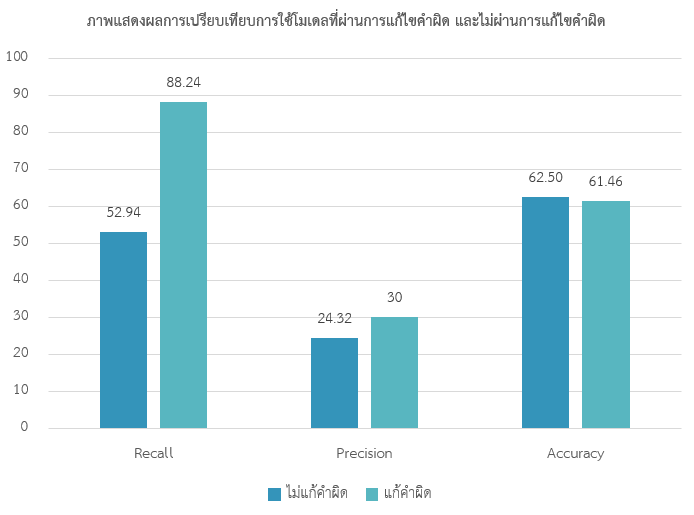
\includegraphics[scale=0.7]{editcompare}
    \caption{ภาพแสดงผลการเปรียบเทียบการใช้โมเดลที่ผ่านการแก้ไขคำผิด และไม่ผ่านการแก้ไขคำผิด}\label{fig:editcompare}
\end{figure}
    
    จากผลลัพธ์ในตารางที่ \ref{tbl:evasearch2} ได้ค่า Precision อยู่ที่ 24.32 \% ค่า Recall 52.94 \% และมี 
    Accuracy 62.5 \% หลังจากการแก้ไขคำและทำการทดลองมีค่า Precision อยู่ที่ 30 \% ค่า Recall 88.24 \% และ
    ค่า Accuracy อยู่ที่ 61.46 \% จะเห็นได้ว่ามีค่า Precision และ Recall สูงขึ้น แต่มีค่า Accuracy ต่ำลง เมื่อทาง
    ผู้จัดทำได้ตรวจสอบระบบการค้นหาพบว่าระบบการค้นหาค่าความสัมพันธ์ Word2Vec ยังไม่ดีนัก เนื่องจาก 
    Word2Vec ของชุดข้อมูล 6 เล่มนั้นมีจำนวน corpus หรือชุดข้อมูลที่นำไปใช้น้อยเกินไปทำให้ค่าความสัมพันธ์ที่ได้จาก 
    Word2Vec มีค่าใกล้เคียงกัน ดังภาพที่ \ref{fig:scoreword2vec} ซึ่ง ทำให้ได้คำที่ไม่เกี่ยวข้องเข้ามาใช้ในการค้นหา อย่างเลข 6 
    หรือ 2009 ที่ถูกดึงมาใช้ทั้งๆที่ไม่มีความเกี่ยวข้อง ส่งผลให้มีหนังสือเล่มอื่นติดมาด้วย ซึ่งสำหรับคำค้นหาคำนี้ถ้า
    เทียบในระบบใหญ่แล้ว ถ้าคำนี้ไม่ถูกอ่านผิดระบบใหญ่จะสามารถแยกความสำคัญได้ดีมากกว่าระบบเล็ก
    
\begin{figure}[H]
    \centering
    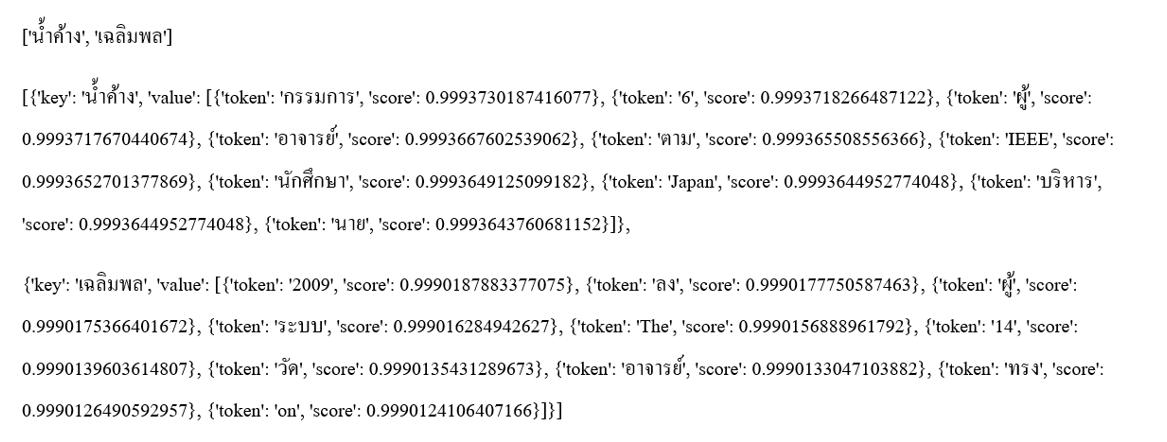
\includegraphics[scale=0.5]{scoreword2vec}
    \caption{ภาพแสดงคะแนนการค้นหาคำเหมือนจากโมเดล word2vec}\label{fig:scoreword2vec}
\end{figure}


ซึ่งถ้าเปรียบเทียบค่า Recall ในแต่ละโมเดลการแก้ไขคำผิด และโมเดลที่ไม่ได้แก้ไขคำผิด จะพบว่าผลลัพธ์การแก้ไขคำผิดจะช่วย
ให้ได้หนังสือที่ครอบคลุมกับผลลัพธ์มากกว่าไม่แก้คำผิด แต่ด้วยความสามารถของโมเดล 
Word2Vec ทำให้ได้หนังสือที่ไม่เกี่ยวข้องเพิ่มมาด้วยเช่นกัน ส่งผลให้มีค่าความแม่นยำ 
หรือค่า Accuracy ลดลง ดังนั้นทางผู้จัดทำได้ลองทำการเปรียบเทียบการค้นหาโดยใช้ 
Word2Vec และไม่ใช้ Word2Vec เข้ามาช่วย ได้ผลลัพธ์ออกมาดังภาพที่ \ref{fig:word2vecCompare}

\begin{figure}[H]
    \centering
    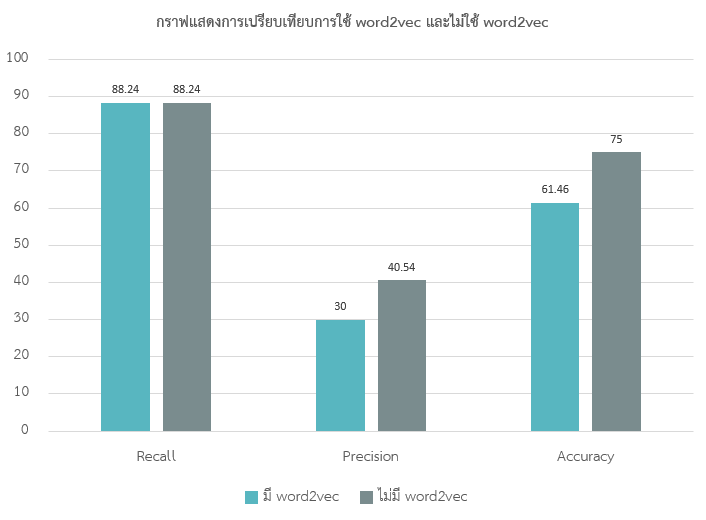
\includegraphics[scale=0.7]{word2vecCompare}
    \caption{ภาพแสดงผลการเปรียบเทียบการใช้ word2vec และไม่ใช้ word2vec}\label{fig:word2vecCompare}
\end{figure}

การค้นหาที่ใช้ Word2Vec จะเป็นการค้นหาที่นำคำค้นหาเข้าโมเดล Word2Vec หลังจากนั้นนำคำที่ได้ไปค้นหาคะแนน TF-IDF เพื่อนำไปหาหนังสือที่มีคะแนนความสัมพันธ์กับคำค้นหาโดยเรียงลำดับจากมากไปน้อย 
ส่วนการค้นหาที่ไม่ใช้ Word2Vec จะเป็นการค้นหาโดยการนำคำค้นหาไปหาคะแนน TF-IDF โดยไม่ผ่านโมเดล Word2Vec
จากภาพที่ \ref{fig:word2vecCompare}  จะเห็นได้ว่า การใช้ Word2Vec ทำให้ประสิทธิภาพในการค้นหาลดลง ถึงแม้ผลลัพธ์ความครอบคลุมของหนังสือที่ถูกต้อง (recall) จะมีค่าเท่ากัน 
แต่ก็มีจำนวนหนังสือที่ไม่เกี่ยวข้องเข้ามาเยอะกว่าเมื่อเทียบการค้นหาแบบใช้ TF-IDF เพียงอย่างเดียว

นอกจากนี้ทางผู้จัดทำได้ทำการเปรียบเทียบประเภทของคำที่ใช้ในการค้นหากับการใช้โมเดล Word2Vec 
พบว่าส่วนใหญ่จะเป็นข้อมูลที่เป็นคำเฉพาะที่มีการผิดพลาดเยอะ
ซึ่งเมื่อได้ลองนำข้อมูลค้นหาที่เป็นคำเฉพาะออกพบว่า ค่า Accuracy เพิ่มขึ้นเป็น 79.17 \% ค่า recall 87.5 \% และค่า Precision 43.75 \% 
รวมถึงคำนวนจากตารางที่ \ref{tbl:evasearchnoname2} และเมื่อเปรียบเทียบกับตารางที่ \ref{tbl:evasearchnoname} จะเห็นได้ชัดว่าการแก้ไขคำผิดส่งผลกับการค้นหาเป็นอย่างมาก

\begin{table}[H]
    \caption{ตารางแสดงผลการค้นหาจากชุดข้อมูล 6 เล่มที่ไม่ผ่านการแก้ไขคำผิดจากมนุษย์แบบไม่มีคำเฉพาะ}\label{tbl:evasearchnoname}
    \begin{tabular}{|c|c|c|}
    \hline
                & TRUE & FALSE \\ \hline
    POSITION & 4   & 13   \\ \hline
    NEGATIVE & 4   & 27   \\ \hline
    \end{tabular}
    \end{table}
    $Recall = 50 \%$ , $Precision = 23.53 \%$ , $Accuracy = 64.6 \%$

\begin{table}[H]
    \caption{ตารางแสดงผลการค้นหาจากชุดข้อมูล 6 เล่มที่ไม่ผ่านการแก้ไขคำผิดจากมนุษย์แบบไม่มีคำเฉพาะ}\label{tbl:evasearchnoname2}
    \begin{tabular}{|c|c|c|}
    \hline
                & TRUE & FALSE \\ \hline
    POSITION & 7   & 9   \\ \hline
    NEGATIVE & 1   & 31   \\ \hline
    \end{tabular}
    \end{table}
    $Recall = 87.5 \%$ , $Precision = 43.75 \%$ , $Accuracy = 79.17 \%$



\subsection{ผลการเปรียบเทียบประสิทธิภาพเวลาในการค้นหา}
ทางผู้จัดทำได้ทำการทดสอบการค้นหาโดยกำหนด คำ 3 คำค้น ให้กับเจ้าหน้าที่บรรณารักษ์และบุคคลธรรมดา 
2 คน โดยกำหนดขอบเขตในการค้นหาหนังสือ 6 เล่ม ซึ่งบุคคลภายนอกที่ใช้ระบบค้นหาของโปรเจคนี้ คนที่ 1 
สามารถระบุหนังสือที่มีเนื้อตรงกับคำค้นหาได้ภายใน 1 นาที ในการค้นหา 3 คำค้นหา และเจอหน้าที่มีคำค้นหา 
3 คำภายใน 11 นาที และคนที่ 2 สามารถระบุหนังสือที่มีเนื้อตรงกับคำค้นหาได้ภายใน 1 นาทีในการค้นหา 3 
คำค้นหา และเจอหน้าที่มีคำค้นหา 3 คำภายใน 9 นาที เมื่อเปรียบเทียบกับเจ้าหน้าที่บรรณารักษ์ที่เปิด
ค้นหาด้วยวิธีการปกติ ทำให้ต้องลองสุ่มหนังสือทุกเล่มจนกว่าจะเจอหนังสือที่มีคำค้นหาทั้ง 3 ซึ่งทำให้ใช้เวลาไปถึง 11 นาที
ถ้าดูโดยภาพรวมแล้วการใช้เว็บกับการค้นหาจากหนังสืออาจจะดูใช้เวลาใกล้เคียงกัน แต่หลังจากที่สอบถามเจ้าหน้าที่บรรณารักษ์พบ
ว่าส่วนใหญ่เสียเวลาให้กับการเปิดหนังสือสุ่มเล่มประมาณ 6 นาที เนื่องจากไม่รู้ว่าควรจะเปิดจากเล่มไหน
 

\section{ผลลัพธ์จากการดำเนินงานในส่วนของการทำเว็บไซต์}
\subsection{การประเมินการใช้งานของเว็บไซต์}
\begin{table}[H]
    \caption{ตารางแสดงผลการประเมินการทดสอบเว็บไซต์}\label{tbl:test2}
    \begin{tabular}{|p{0.3\linewidth}|l|l|p{0.35\linewidth}|}
    \hline
    \multicolumn{4}{|c|}{ตารางประเมิน Test}                                                               \\ \hline
    \multicolumn{1}{|c|}{}                         & \multicolumn{2}{c|}{ผลลัพธ์} & \multicolumn{1}{c|}{} \\ \cline{2-3}
    \multicolumn{1}{|c|}{\multirow{-2}{*}{เกณฑ์การประเมิน}} &
        \multicolumn{1}{c|}{ผ่าน} &
        \multicolumn{1}{c|}{ไม่ผ่าน} &
        \multicolumn{1}{c|}{\multirow{-2}{*}{หมายเหตุ}} \\ \hline
    1. สามารถเข้าสู่ระบบและออกจาก ระบบได้          & \cellcolor[HTML]{B5E645}  &  &                       \\ \hline
    2. สามารถเพิ่มเอกสารเข้าสู่ระบบได้             & \cellcolor[HTML]{B5E645}  &  &                       \\ \hline
    3. สามารถแก้ไขรายละเอียดเอกสารที่อยู่ในระบบได้ & \cellcolor[HTML]{B5E645}  &  &                       \\ \hline
    4. สามารถตรวจสอบและแก้ไขคำที่เพิ่มเข้ามาในระบบในขั้นตอนเพิ่มเอกสารได้ & 
        \cellcolor[HTML]{B5E645} & 
        & ข้อสังเกตเกี่ยวกับการ Re-index ว่ามีผลต่อการค้นหาแบบ Real-time หรือไม่
        \\ \hline
    5. สามารถลบเอกสารที่อยู่ในระบบได้              & \cellcolor[HTML]{B5E645}  &  &                       \\ \hline
    6.   สามารถค้นหาข้อมูลเอกสารภายในระบบได้       & \cellcolor[HTML]{B5E645}  &  &                       \\ \hline
    7.   สามารถเรียกดูเอกสารที่ต้องการได้          & \cellcolor[HTML]{B5E645}  &  &                       \\ \hline
    \end{tabular}
    \end{table}
\subsection{การประเมินความพึงพอใจของบรรณารักษ์ต่อการออกแบบ UX/UI}
\begin{table}[H]
\caption{ตารางประเมินความพึงพอใจการออกแบบ UX/UI}\label{tbl:uxuieva}
\begin{flushleft}
\begin{tabular}{|p{0.13\linewidth}|p{0.17\linewidth}|p{0.17\linewidth}|p{0.17\linewidth}|p{0.17\linewidth}|c|}
    \hline
                        & \multicolumn{1}{c|}{4}                                                                                                 & \multicolumn{1}{c|}{3}                                                                                   & \multicolumn{1}{c|}{2}                                                                                        & \multicolumn{1}{c|}{1}                                                                        & คะแนนที่ได้ \\ \hline
ความสมบูรณ์ของข้อมูล    & ข้อมูลมีความสมบูรณ์   ชัดเจนทำให้เข้าใจความหมายที่ต้องการจะสื่อได้เป็นอย่างดี                                            &  มีข้อมูลที่ชัดเจน   และแม่นยำในบางครั้ง และสามารถแสดงความหมายที่ต้องการจะสื่อได้บ้าง                     &ข้อมูลมีความแม่นยำ   และชัดเจนบ้าง                                                                            & มีข้อมูลที่ไม่ชัดเจน   ไม่ครบ สื่อความหมายได้ไม่ดี                                            & 3           \\ \hline
การออกแบบ           & มีการออกแบบที่เน้นความสำคัญและจัดวางองค์ประกอบ   สี เสียง และการเคลื่อนไหว(animation) ได้อย่างเหมาะสม                            &  มีการจัดหน้า   และองค์ประกอบทำให้เห็นใจความสำคัญของเนื้อหา มีการใช้การเคลื่อนไหว(animation) บ้าง                    & การวางหน้าและการจัดองค์ประกอบมีความไม่เหมาะสม   มีการใช้การเคลื่อนไหว(animation) เข้ามาช่วยบ้าง                               & การวางหน้าและการจัดองค์ประกอบมีความไม่เหมาะสมและไม่มีการใช้  การเคลื่อนไหว(animation) เข้ามาช่วยในการใช้งาน & 4           \\ \hline
การใช้งาน            &  ผู้ใช้สามารถใช้งานปุ่มหรือย้ายไปยังหน้าต่างๆได้อย่างง่ายดาย   แต่มีลิ้งค์(Link) ที่พาไปผิดหน้าอย่างมากหนึ่งลิ้งค์(Link) หรือไม่มีเลย                &  ผู้ใช้สามารถใช้งานปุ่มหรือย้ายไปยังหน้าต่างๆได้อย่างง่ายดาย   แต่มีลิ้งค์(Link) ที่พาไปผิดหน้าอย่างมากสองลิ้งค์(Link)            &ผู้ใช้มีความสับสนในการใช้ปุ่ม   หรือการย้ายไปยังหน้าต่างๆ บางครั้ง และมีลิ้งค์(Link) ที่พาไปผิดหน้าอย่างมากสามลิ้งค์(Link)                      & ผู้ใช้เกิดความสับสนในปุ่มหรือลิ้งค์(Link) ที่ย้ายไปหน้าต่างๆ                                         & 4           \\ \hline
การใช้ภาษา           & มีการใช้คำผิดหรือภาษาที่ไม่เหมาะสมอย่างมาก   1 จุด                                                               &  มีการใช้คำผิดหรือภาษาที่ไม่เหมาะสมอย่างมาก   2 จุด                                                &มีการใช้คำผิดหรือภาษาที่ไม่เหมาะสมอย่างมาก 3 จุด                                                                 & มีการใช้คำผิดหรือภาษาที่ไม่เหมาะสมมากกว่า 4 จุด                                               & 4           \\ \hline
\end{tabular}
\end{flushleft}
\end{table}

\subsection{หน้าหลัก}
\begin{figure}[H]
    \centering
    
\includegraphics[scale=0.2]{web1}
    \caption{ภาพแสดงหน้าเว็บหลัก}\label{fig:web1}
\end{figure}

\subsection{การเข้าสู่ระบบเว็บไซต์}
\begin{figure}[H]
    \centering
    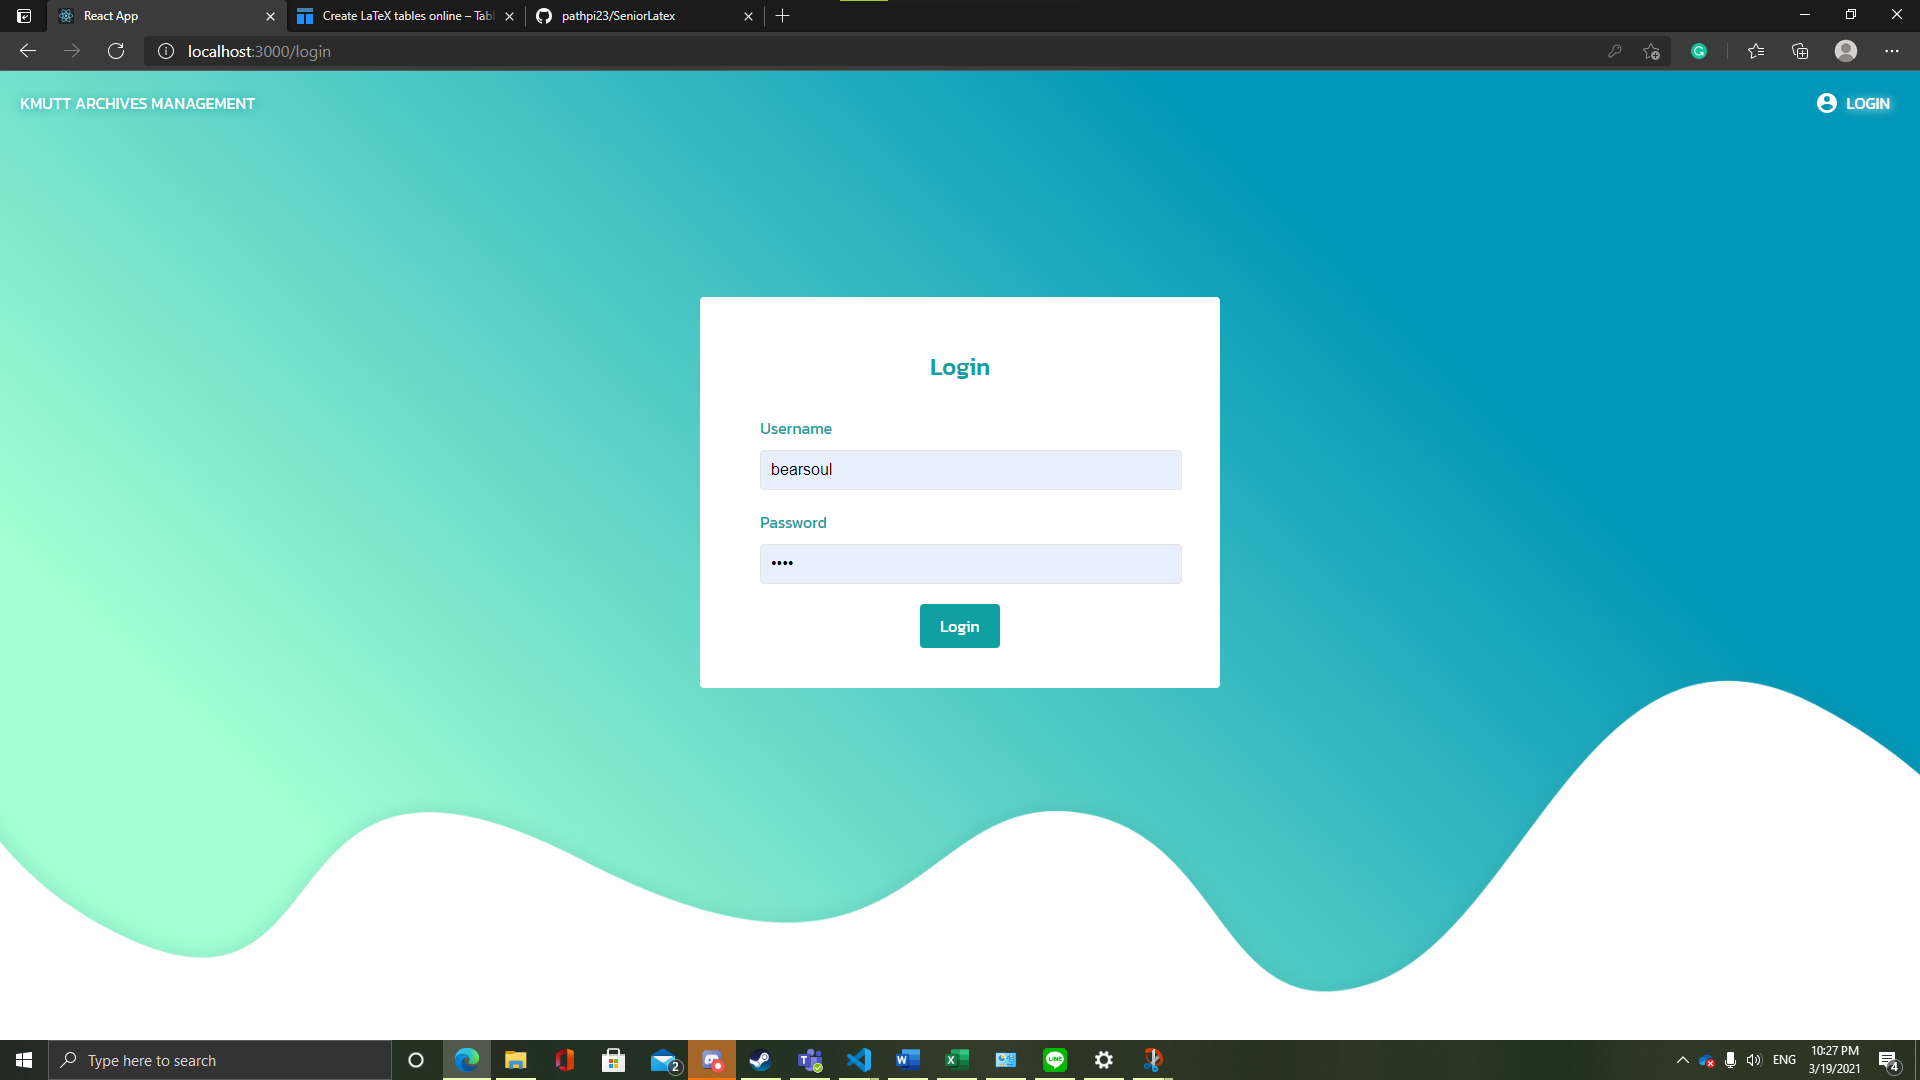
\includegraphics[scale=0.2]{weblogin}
    \caption{ภาพแสดงหน้าเข้าสู่ระบบ}\label{fig:weblogin}
\end{figure}
การเข้าสู่ระบบในเว็บไซต์เราได้ใช้ JSON Web Token (JWT) ในการดูสิทธิ์การเข้าใช้ระบบโดยที่เมื่อผู้ใช้งานเข้าสู่ระบบด้วยรหัสผู้ใช้งานและรหัสผ่านที่ถูกต้องNode JS ก็จะคืน Token ที่ถูกเข้ารหัสไว้กลับไปให้ทางเครื่องผู้ใช้งานเก็บใน local storage เพื่อที่จะเป็นการบ่งบอกสิทธิ์การใช้งาน API ที่เหลือทั้งหมดไม่ว่าจะเป็นการค้นหาข้อมูล เพิ่มข้อมูลหนังสือ แก้ไขข้อมูลหนังสือ หรือลบข้อมูลหนังสือออกจากระบบ ถ้าผู้ใช้งานไม่ได้ส่ง Token มาด้วยหรือ Token นั้นมีการดัดแปลงแก้ไขระบบจะทำการลบ Token ภายในเครื่องทึ้งและทำการออกจากระบบโดยทันที

\subsection{การเพิ่มหนังสือเข้าสู่ระบบฐานข้อมูล}
เนื่องจากการเพิ่มหนังสือเข้าสู่ระบบมีขั้นตอนจำนวนมากและใช้เวลานานจึงแบ่งการรอประมวลผลเป็นส่วนของการเพิ่มข้อมูลของหนังสือ ส่วนของการแก้ไขและตรวจสอบคำก่อนนำเข้าสู่ระบบ ส่วนของการตรวจสอบแก้ไขคำสำคัญ ซึ่งผู้ใช้งานไม่จำเป็นต้องรอภายในหน้าเพิ่มหนังสือสามารถไปทำงานฟังก์ชั่นอื่นได้ตามปกติและเมื่อเสร็จกระบวนการเหล่านี้เสร็จจะสามารถกลับมาดำเนินการเพิ่มข้อมูลต่อได้โดยการกดที่หน้าแสดงสถานะ และกลับเข้าสู่กระบวนการเพิ่มข้อมูลหนังสือ
\subsubsection{เพิ่มข้อมูลของหนังสือ}
\begin{figure}[H]
    \centering
    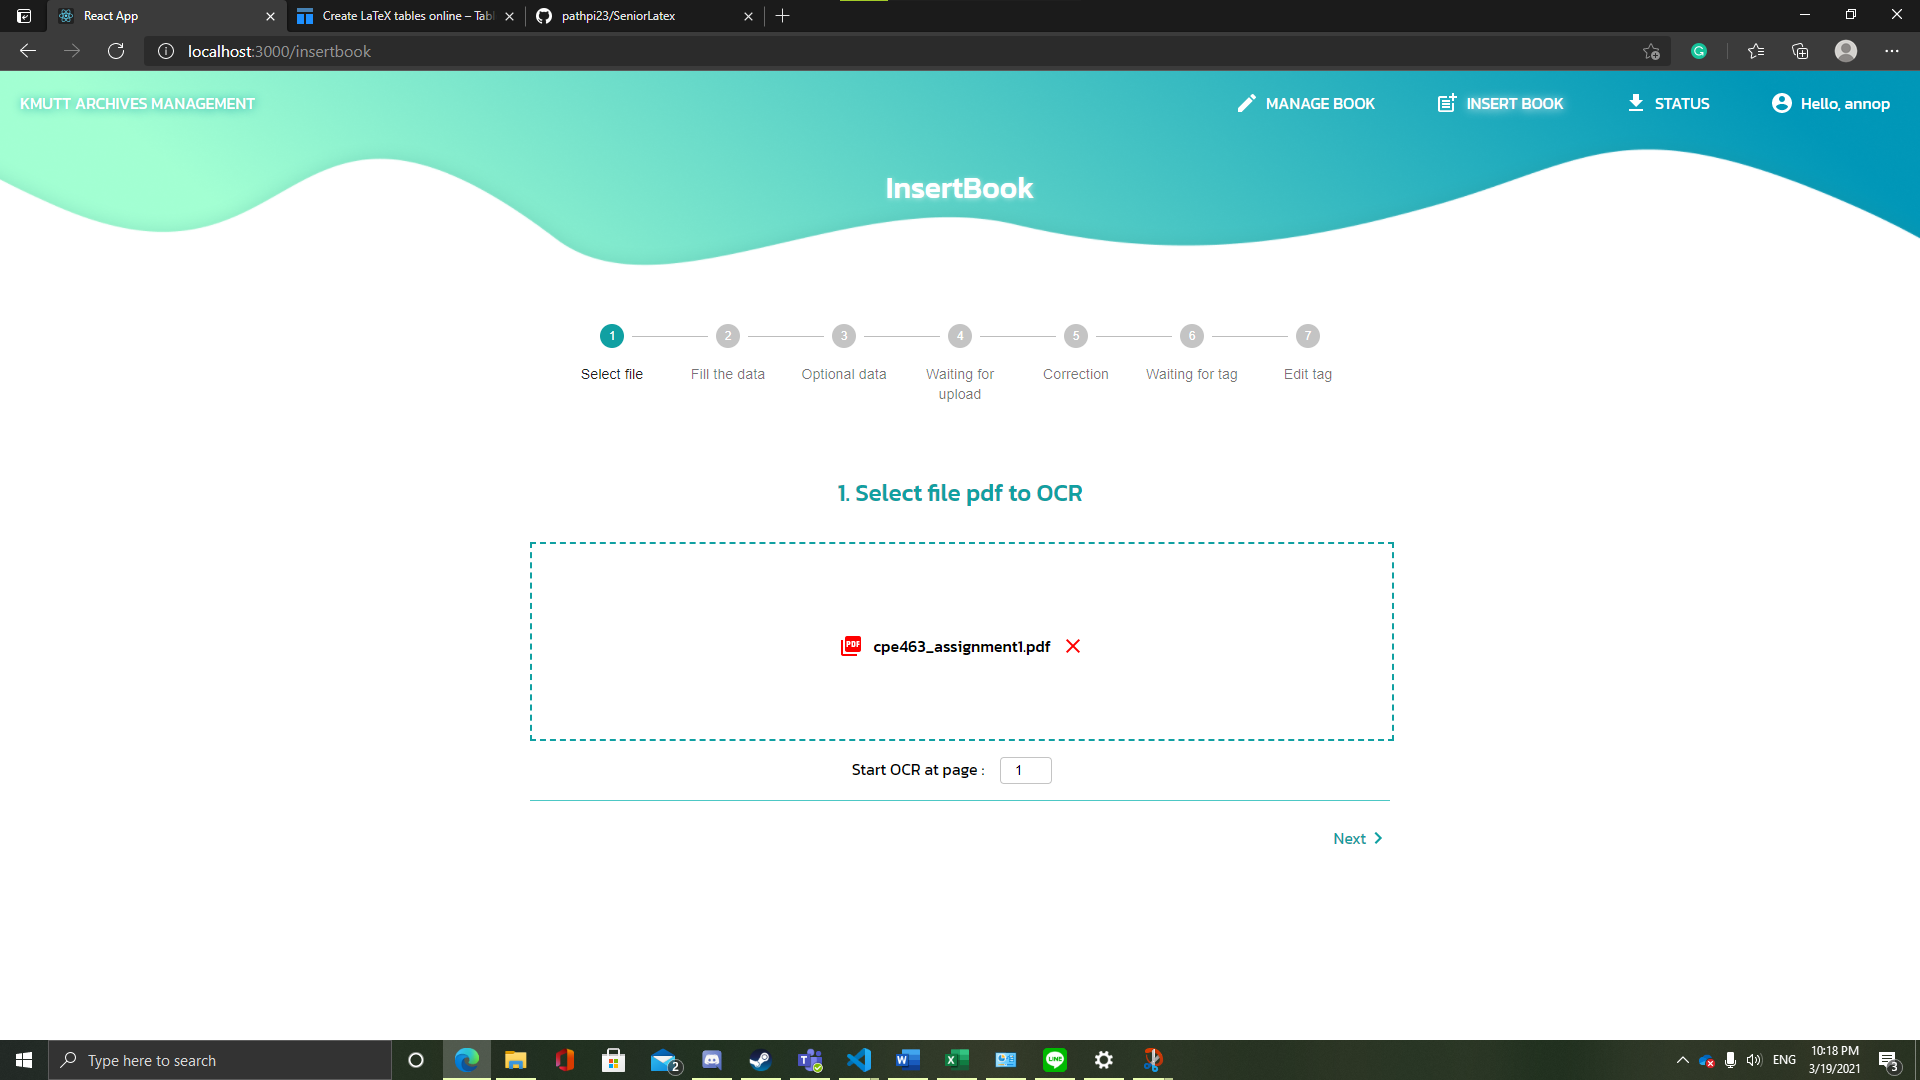
\includegraphics[scale=0.2]{webinsert}
    \caption{ภาพแสดงขั้นตอนการเพิ่มหนังสือขั้นตอนการเพิ่มไฟล์}\label{fig:webinsert}
\end{figure}
\begin{figure}[H]
    \centering
    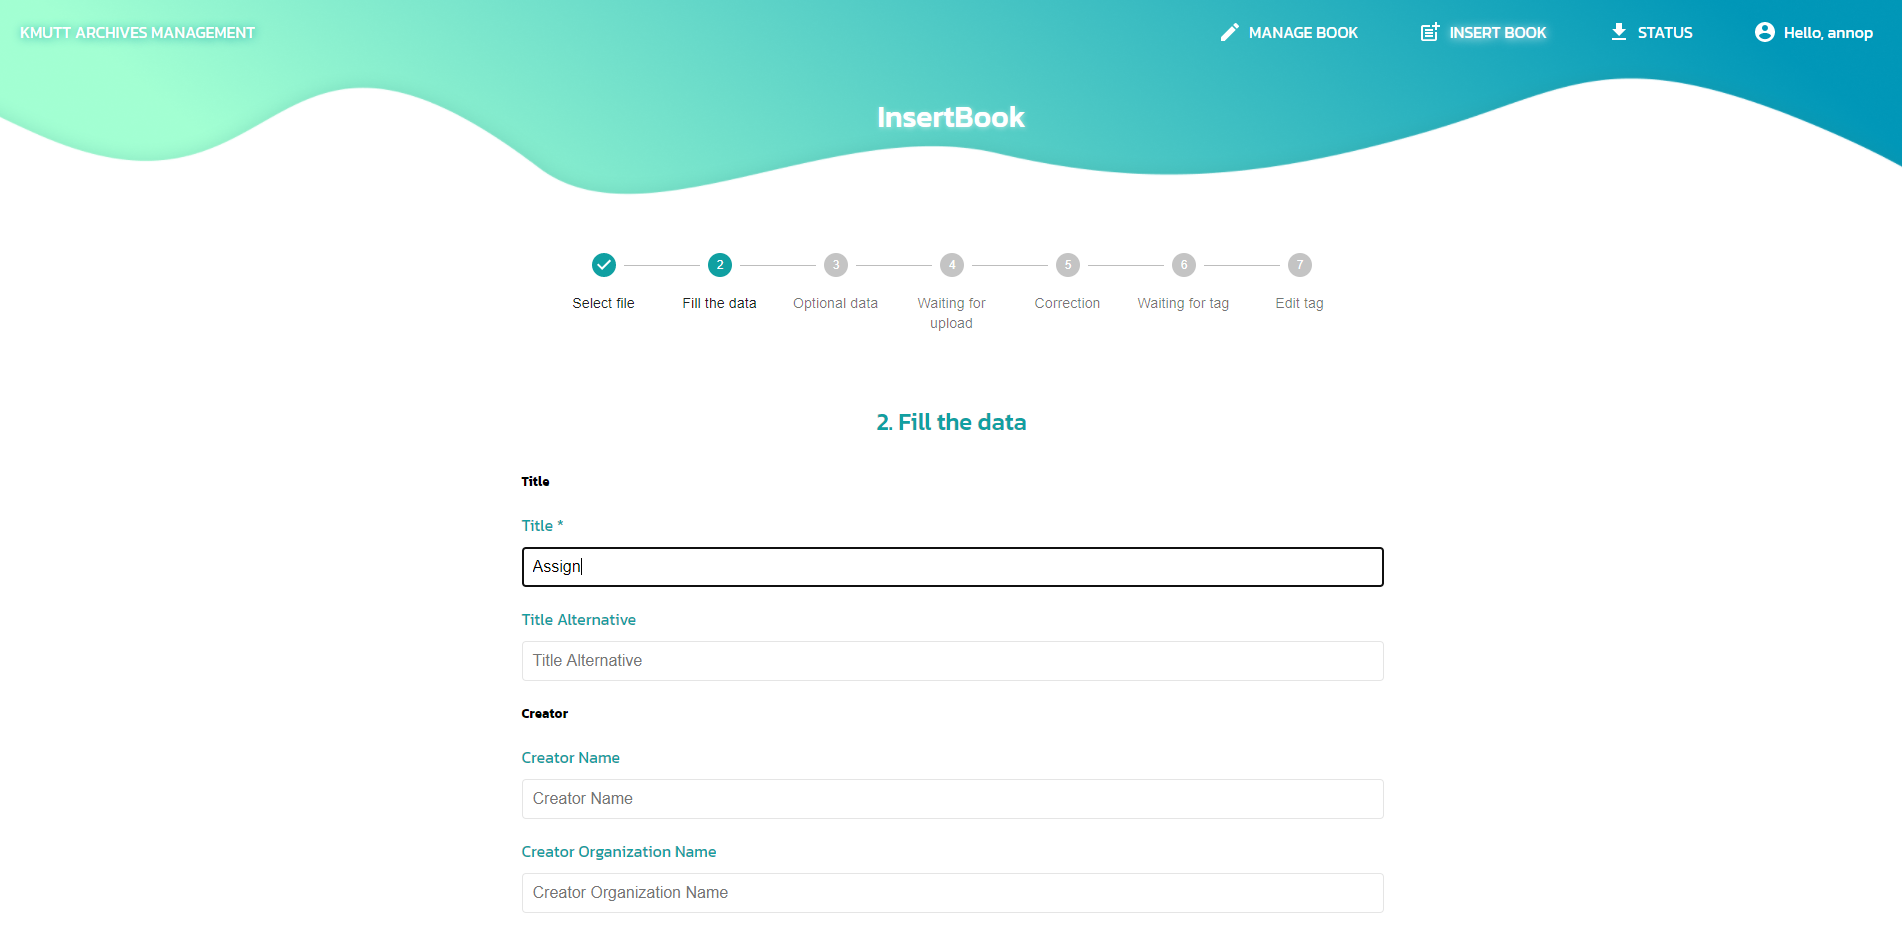
\includegraphics[scale=0.2]{webinsert2}
    \caption{ภาพแสดงขั้นตอนการเพิ่มหนังสือเข้าสู่ระบบขั้นกรอกข้อมูลขั้นที่ 1}\label{fig:webinsert2}
\end{figure}
\begin{figure}[H]
    \centering
    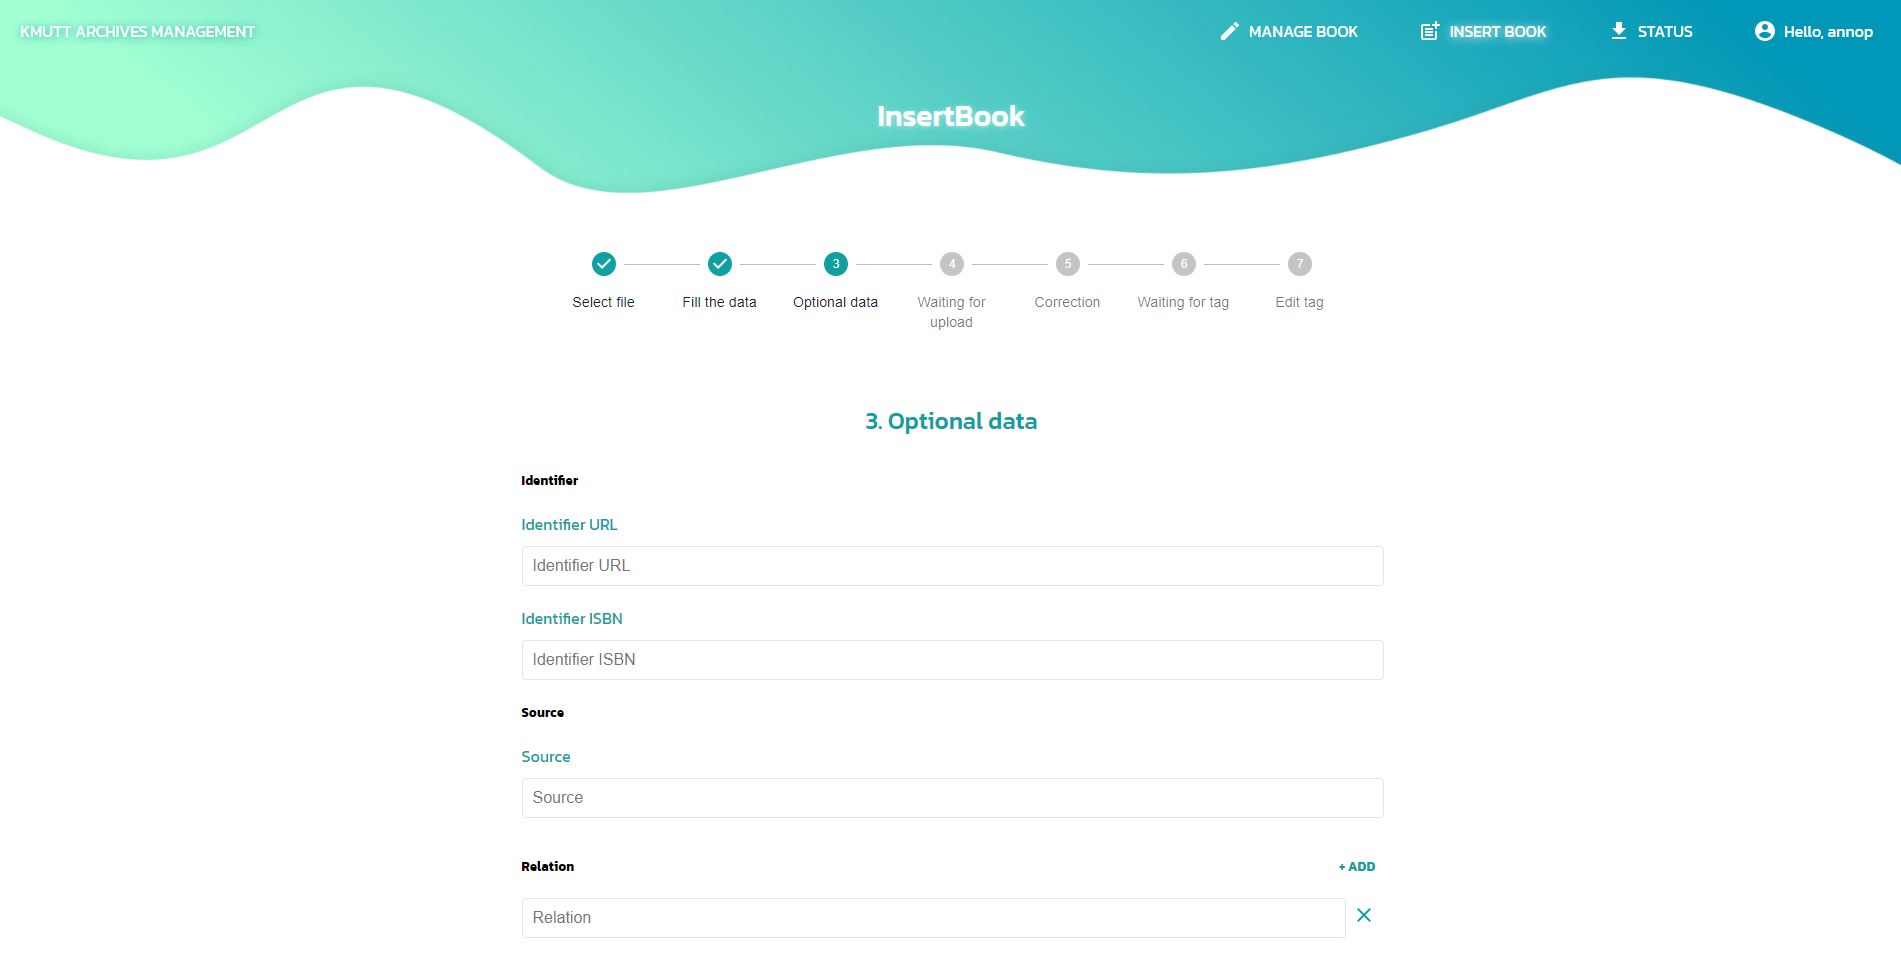
\includegraphics[scale=0.2]{webinsert3}
    \caption{ภาพแสดงขั้นตอนการเพิ่มหนังสือเข้าสู่ระบบขั้นกรอกข้อมูลขั้นที่ 2}\label{fig:webinsert3}
\end{figure}

\begin{figure}[H]
    \centering
    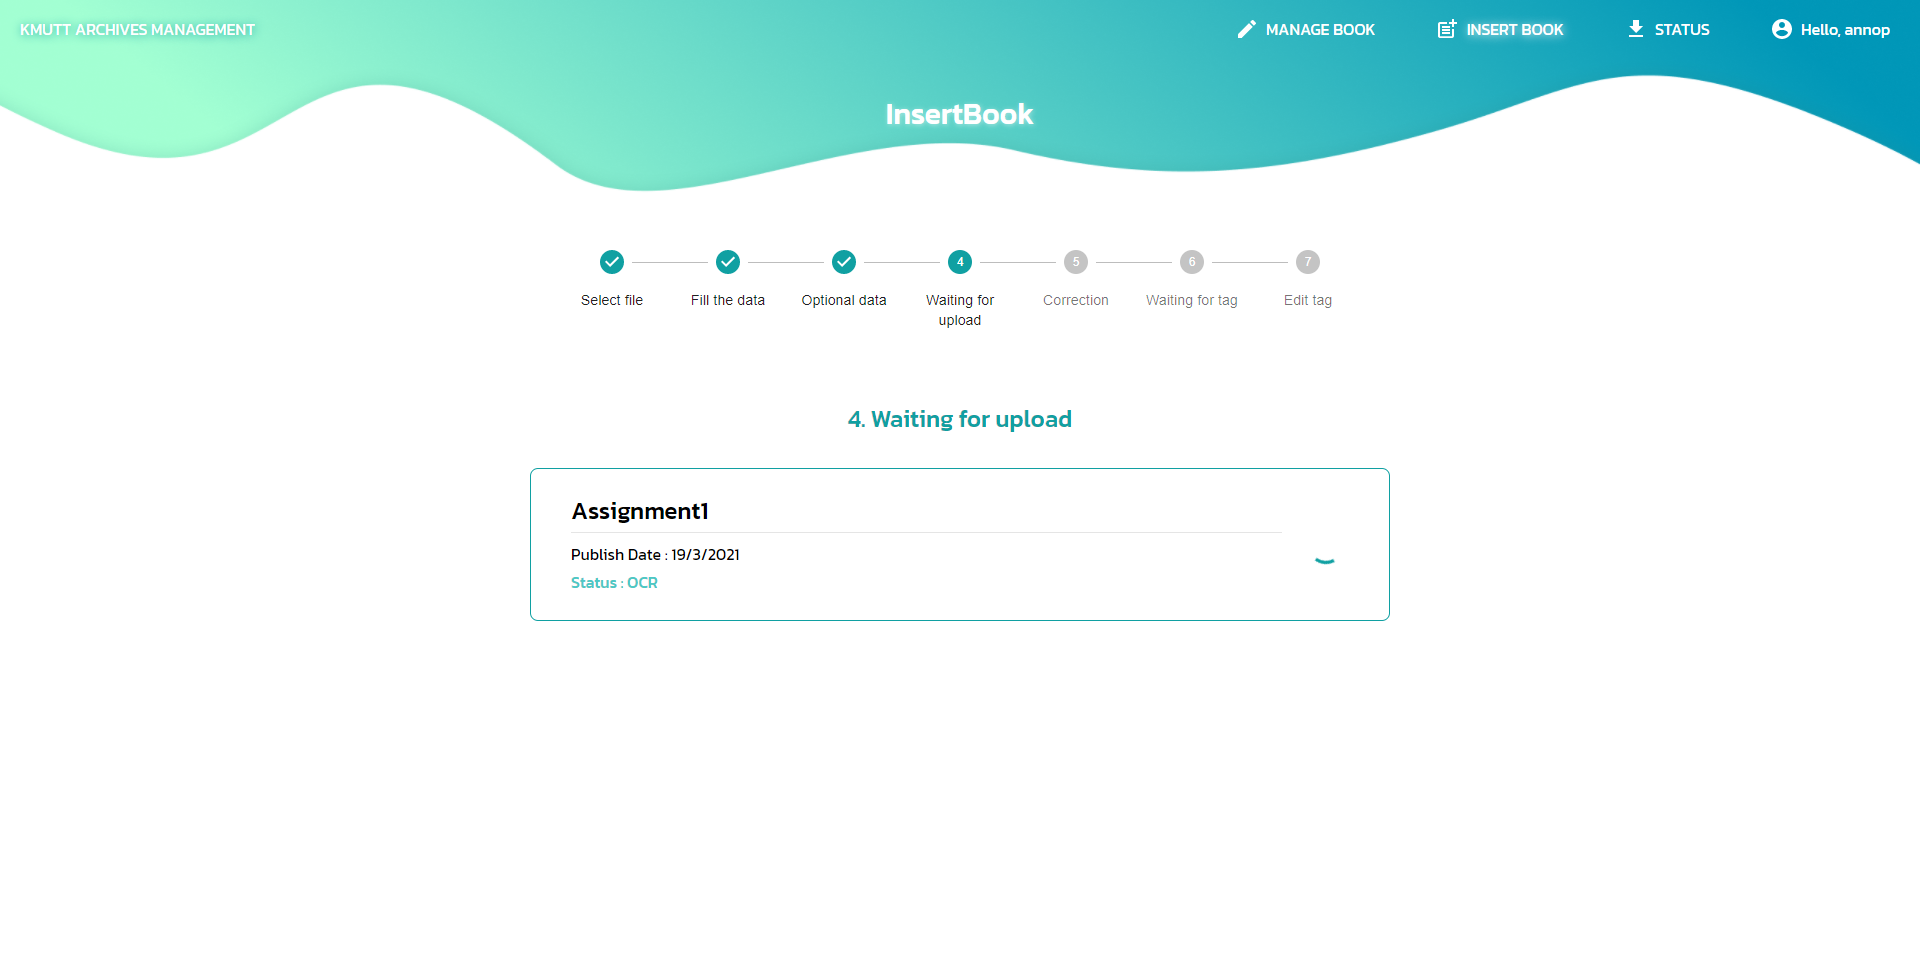
\includegraphics[scale=0.2]{webinsert4}
    \caption{ภาพแสดงขั้นตอนการเพิ่มหนังสือเข้าสู่ระบบขั้นการเตรียมข้อมูล}\label{fig:webdel}
\end{figure}
ในส่วนนี้จะเป็นการใช้ผู้ใช้งานทำการเลือกไฟล์ PDF และกรอกข้อมูลของหนังสือโดยที่เมื่อผู้ใช้งานยืนยันข้อมูลเรียบร้อยแล้วระบบก็จะทำการเพิ่มไฟล์ PDF เพื่อนำไปทำกระบวนการเปลี่ยน PDF เป็นรูปภาพและทำการ OCR และการเตรียมข้อมูลตัวอักษร  เพื่อทำการแปลงข้อมูลออกมาให้ผู้ใช้งาน

\subsubsection{การแก้ไขและตรวจสอบคำก่อนนำเข้าสู่ระบบ}
\begin{figure}[H]
    \centering
    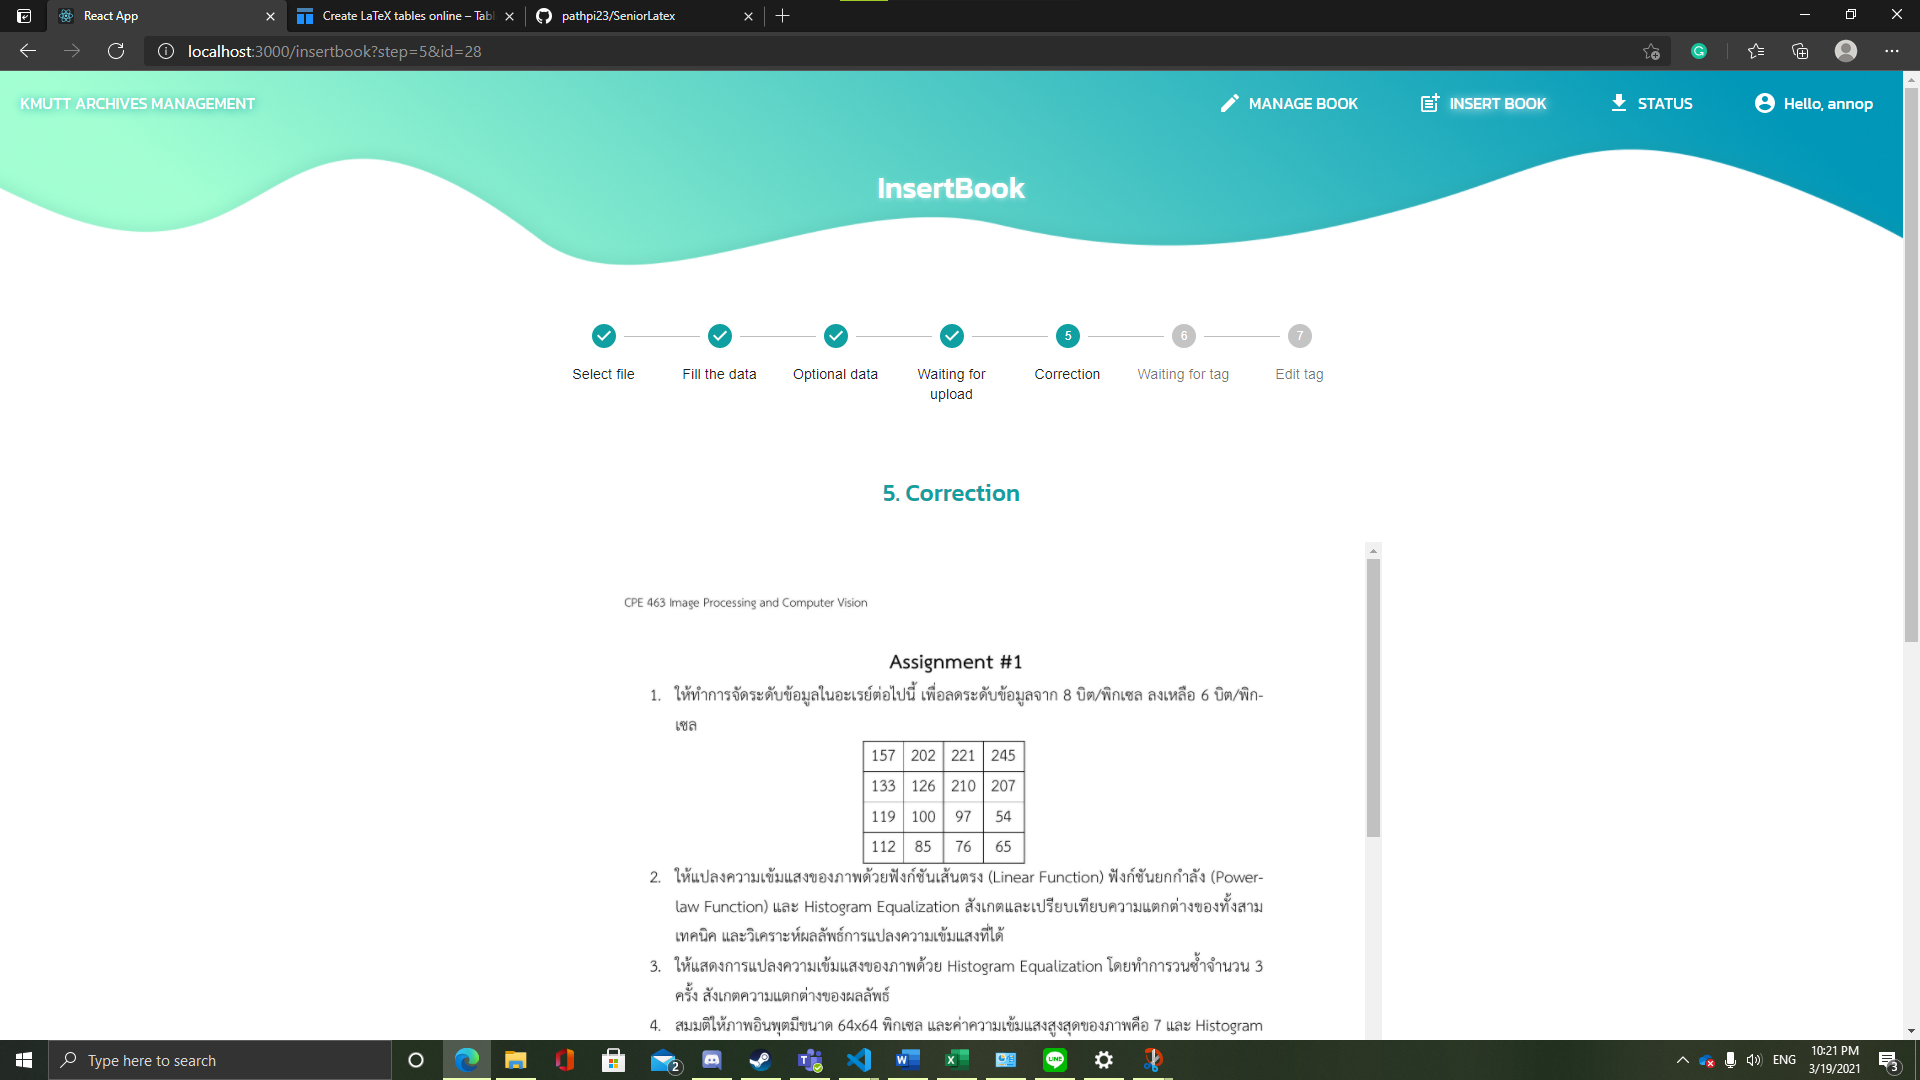
\includegraphics[scale=0.2]{webcorrect}
    \caption{ภาพแสดงขั้นตอนการเพิ่มหนังสือเข้าสู่ระบบขั้นการแก้ไขคำผิด}\label{fig:webcorrect}
\end{figure}

\begin{figure}[H]
    \centering
    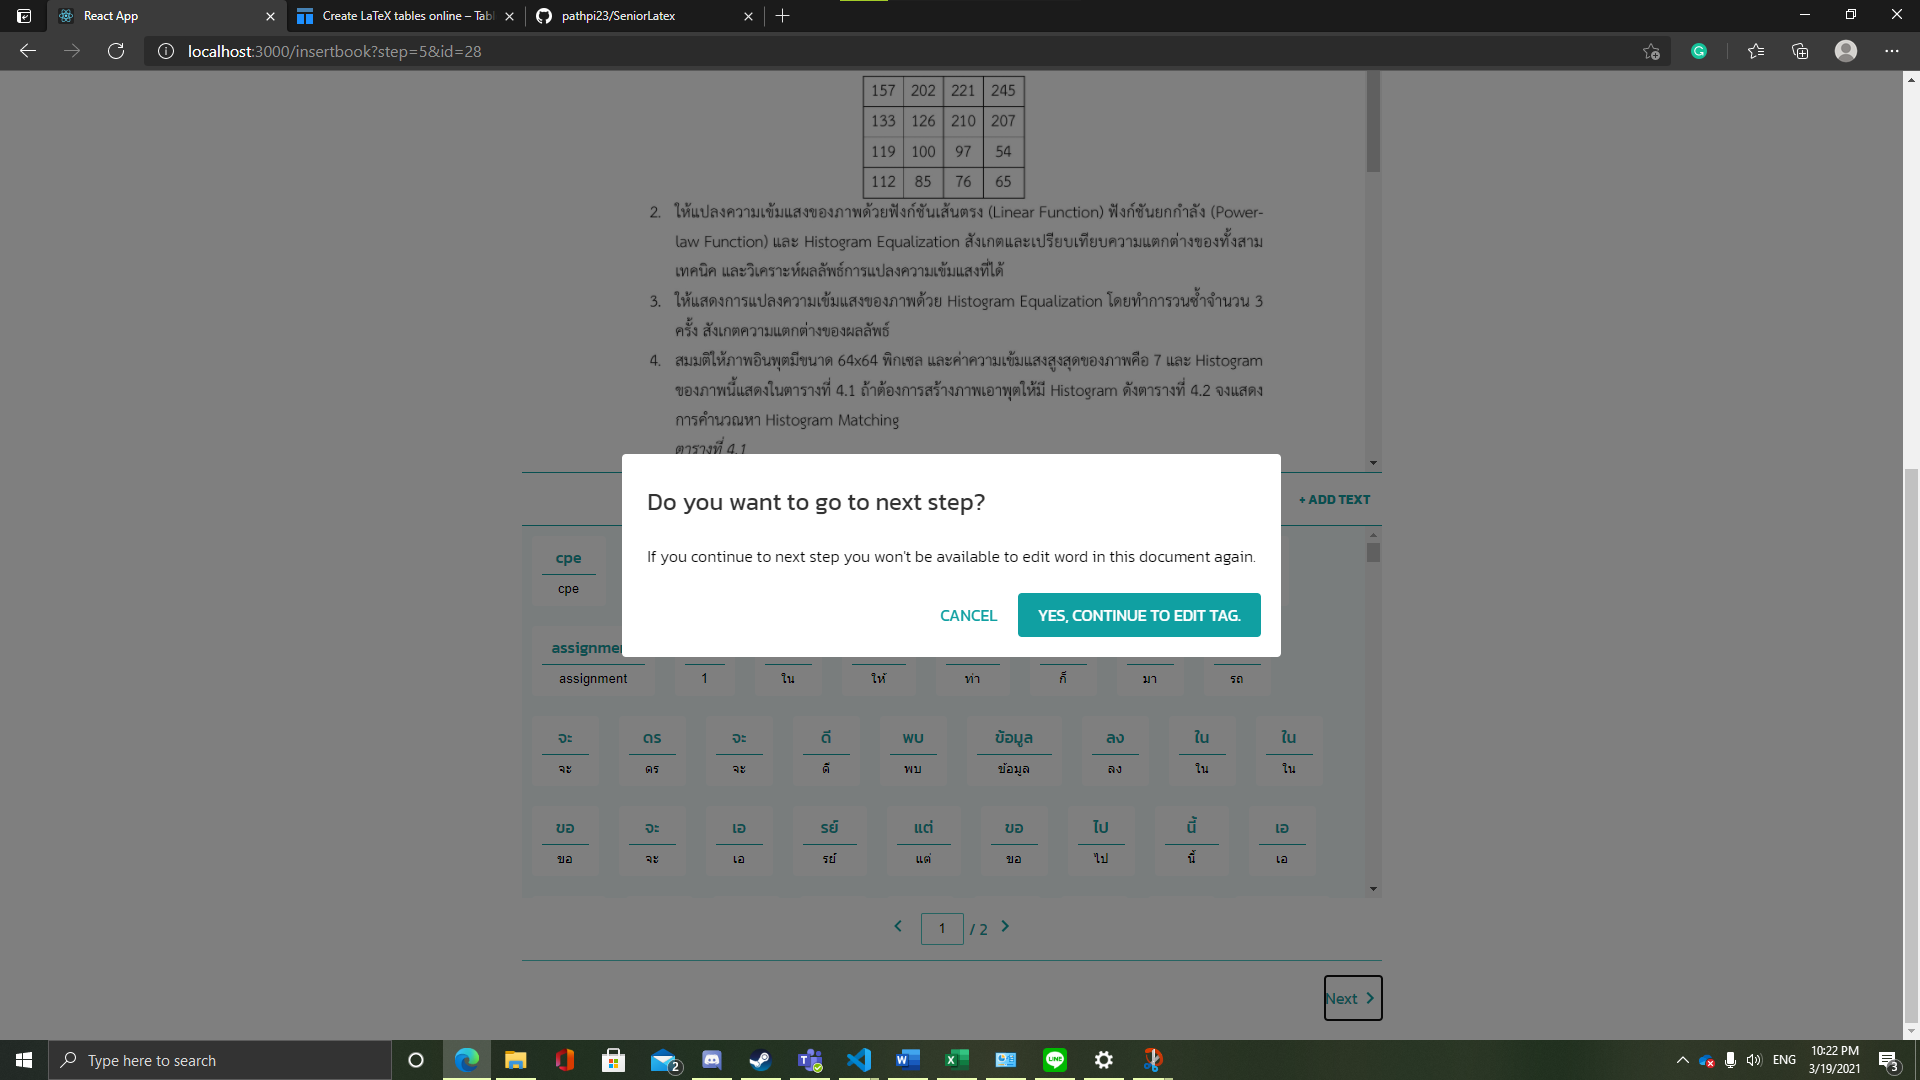
\includegraphics[scale=0.2]{websubmit}
    \caption{ภาพแสดงหน้าต่างยืนยันการแก้คำ}\label{fig:websubmit}
\end{figure}

\begin{figure}[H]
    \centering
    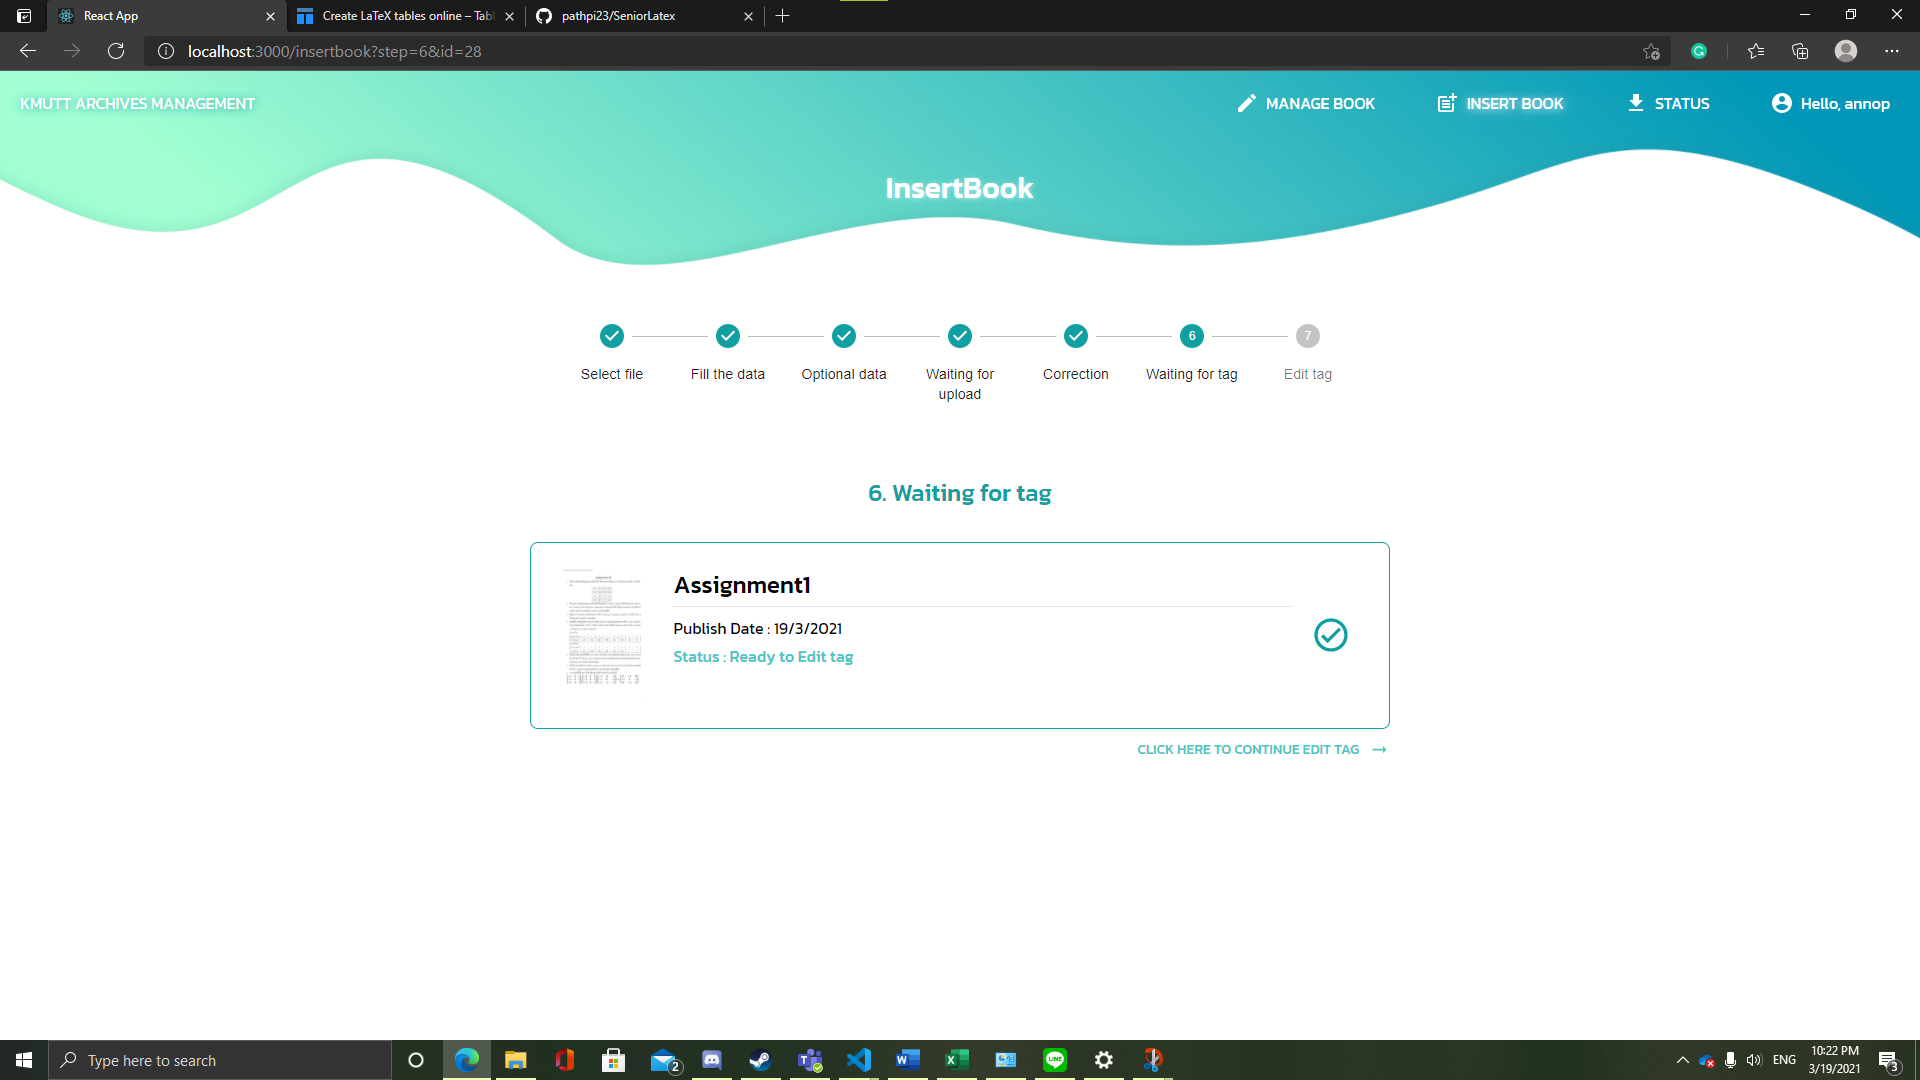
\includegraphics[scale=0.2]{webcheckout}
    \caption{ภาพแสดงขั้นตอนการเพิ่มหนังสือเข้าสู่ระบบขั้นการสร้างคำสำคัญ}\label{fig:webcheckout}
\end{figure}
ในส่วนนี้จะเป็นผลลัพธ์การดำเนินการของการเพิ่มข้อมูลหนังสือ จะมีคำของแต่ละหน้าพร้อมรูปภาพประกอบเพื่อให้ผู้ใช้งานได้ตรวจสอบคำเพิ่มและแก้ไขคำได้อย่างอิสระก่อนจะนำคำเหล่านี้เข้าสู่ระบบและในส่วนนี้ถ้ายืนยันการแก้ไขแล้วจะไม่สามารถมาแก้ไขคำในหนังสือเล่มนี้ในระบบได้อีกโดยถ้ายืนยันแล้วระบบจะทำการเพิ่มคำเหล่านี้เข้าสู่ระบบและทำการคำนวนคะแนน TF-IDF ของคำเหล่านี้ก่อนจะสร้างคำสำคัญของหนังสือเล่มนี้ให้อัตโนมัติ

\subsubsection{การตรวจสอบแก้ไขคำสำคัญ}
\begin{figure}[H]
    \centering
    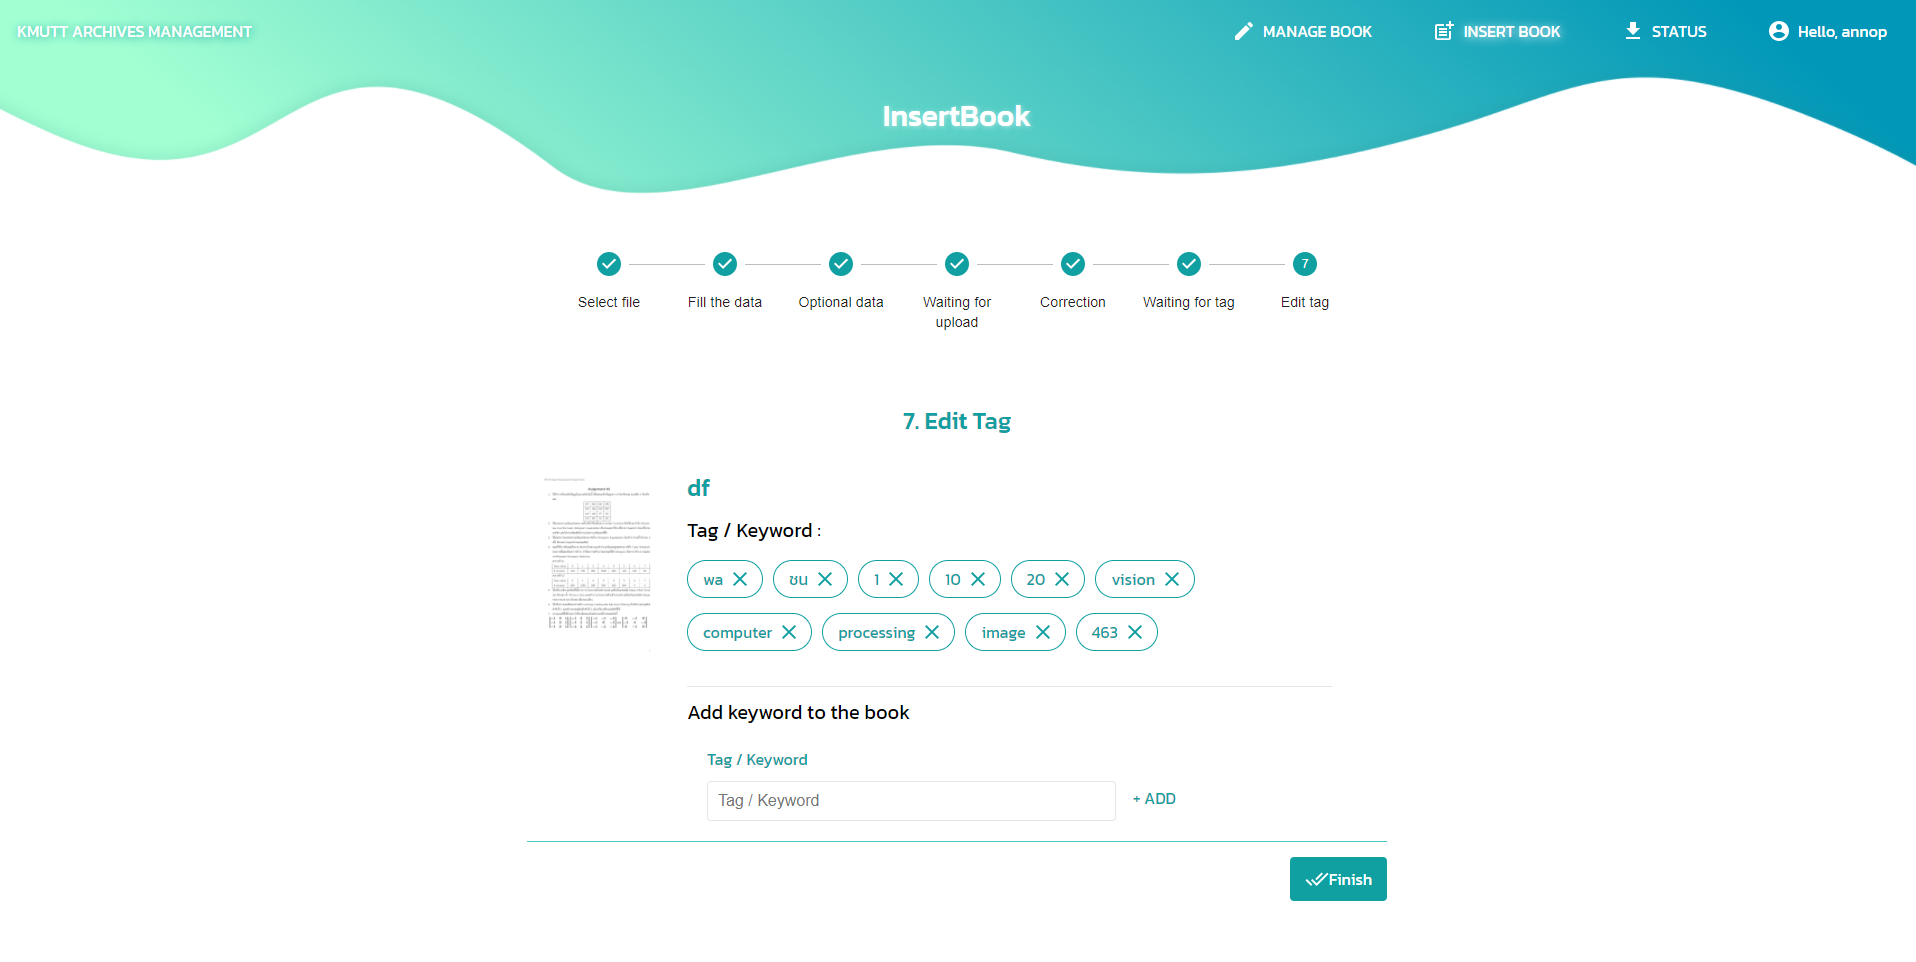
\includegraphics[scale=0.2]{webtag}
    \caption{ภาพแสดงขั้นตอนการเพิ่มหนังสือเข้าสู่ระบบขั้นการแก้ไขคำสำคัญ}\label{fig:webtag}
\end{figure}
ในส่วนนี้จะเป็นผลลัพธ์ของการแก้ไขและตรวจสอบคำก่อนนำเข้าสู่ระบบโดยผู้ใช้งานได้คำสำคัญ ที่ทางระบบทำขึ้นอัตโนมัติเพื่อให้ผู้ใช้งานได้ตรวจสอบเพิ่มลดคำสำคัญ ก่อนจะยืนยันเพิ่มเข้าสู่ระบบ
\subsection{การแสดงสถานะการเพิ่มหนังสือ}
\begin{figure}[H]
    \centering
    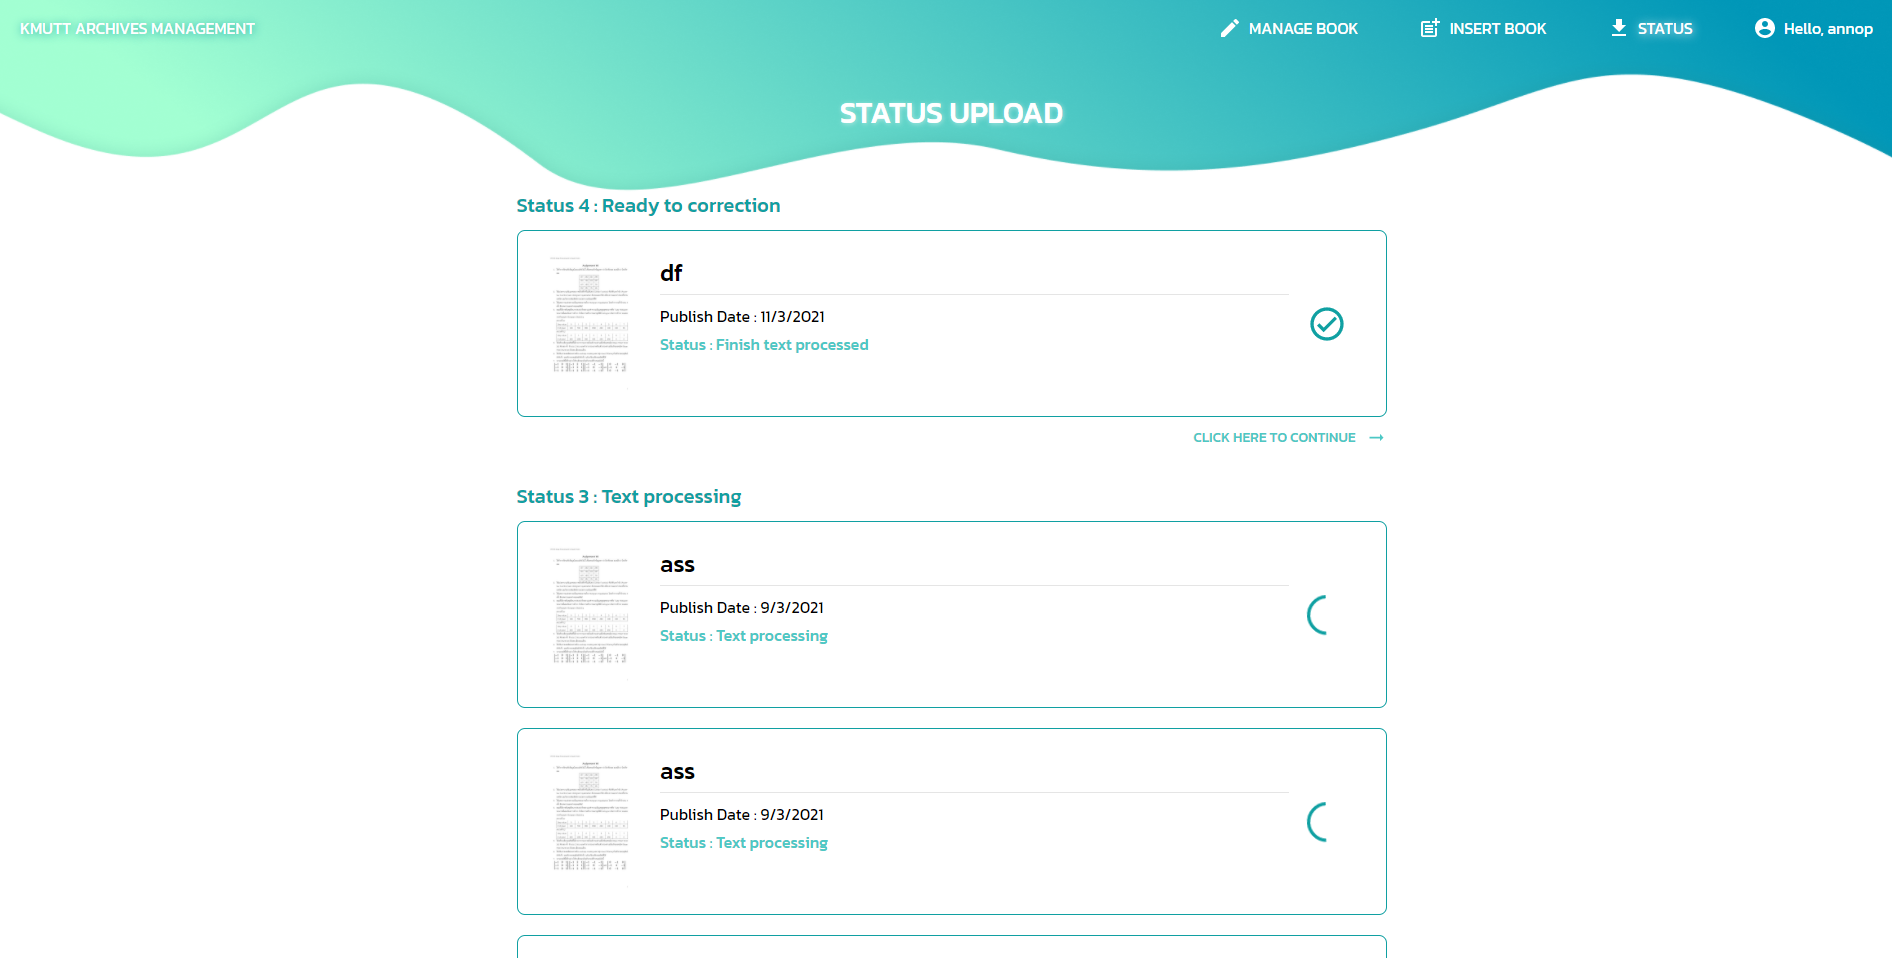
\includegraphics[scale=0.2]{webstatus}
    \caption{ภาพแสดงสถานะของการเพิ่มข้อมูลเข้าสู่ระบบ}\label{fig:webstatus}
\end{figure}

\subsection{การแสดงการค้นหาหนังสือ}
\begin{figure}[H]
    \centering
    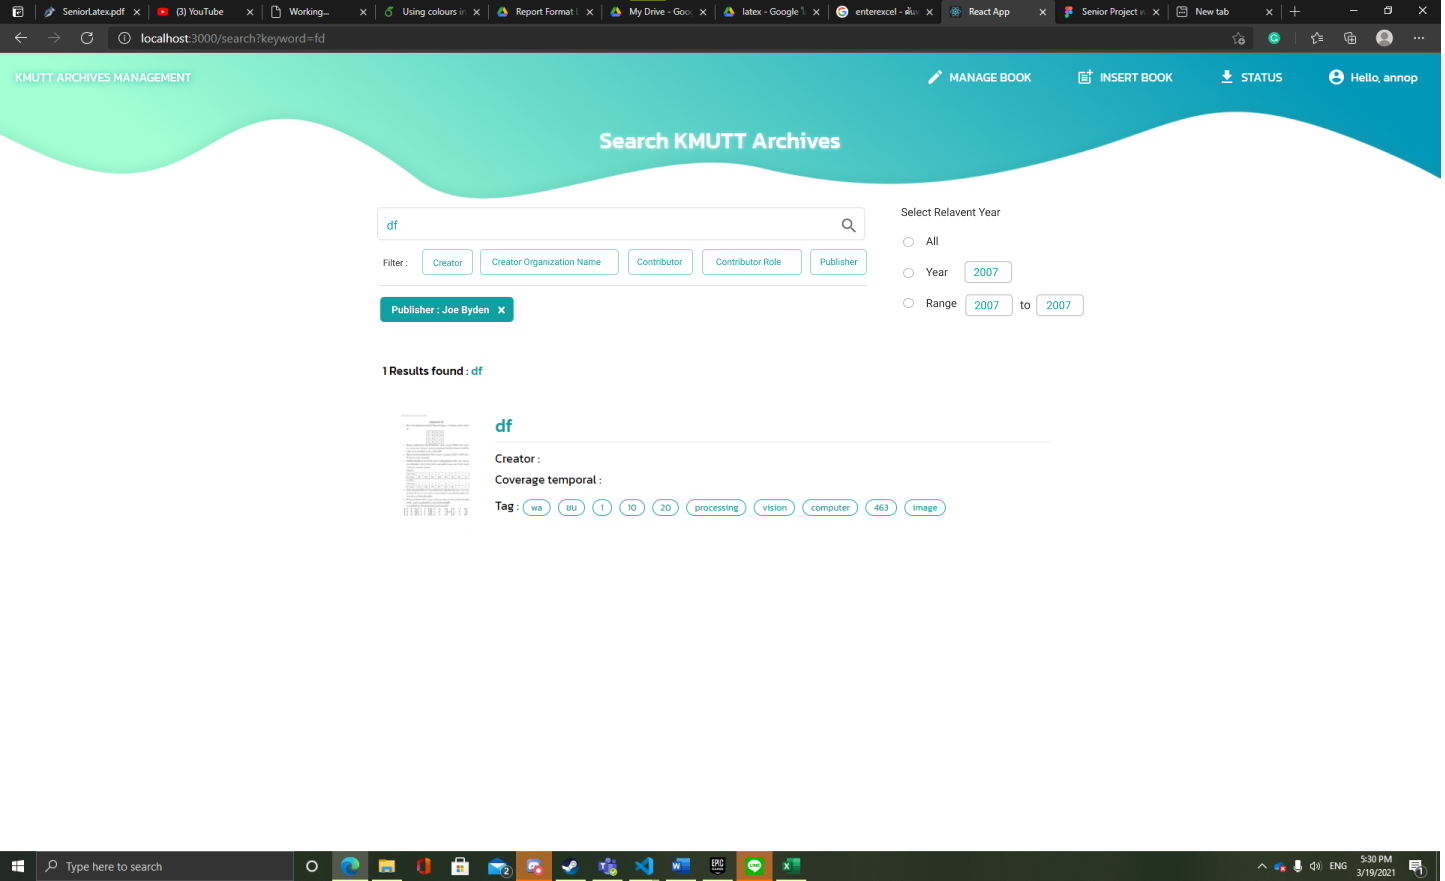
\includegraphics[scale=0.2]{websearch}
    \caption{ภาพแสดงหน้าการค้นหา}\label{fig:websearch}
\end{figure}

\subsection{การแสดงข้อมูลหนังสือ}
\begin{figure}[H]
    \centering
    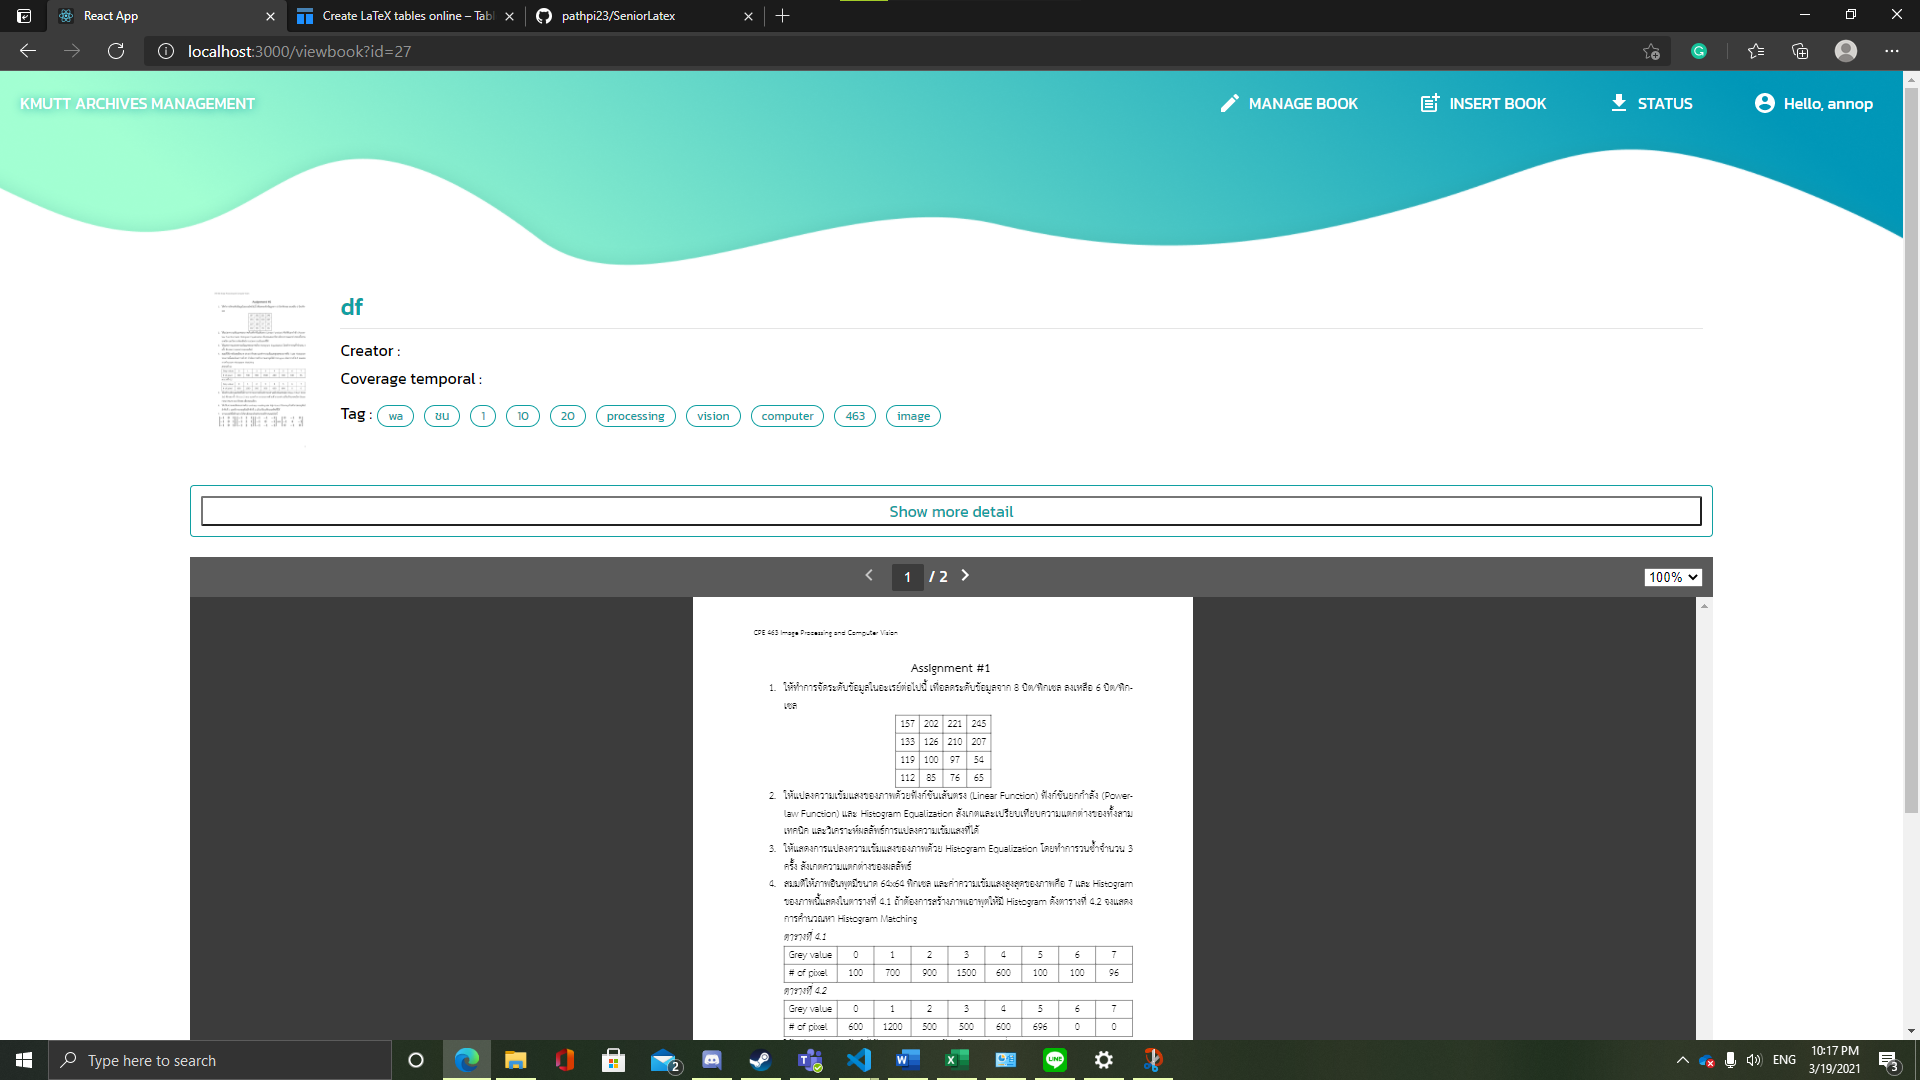
\includegraphics[scale=0.2]{webview}
    \caption{ภาพแสดงหน้าแสดงหนังสือ}\label{fig:webview}
\end{figure}
จะเป็นการแสดงข้อมูลของหนังสือที่อยู่ภายในระบบที่ผู้ใช้งานกรอกเข้ามาในระบบพร้อมทั้งแสดง PDF ที่ถูกอัพโหลดขึ้นมา

\begin{figure}[H]
    \centering
    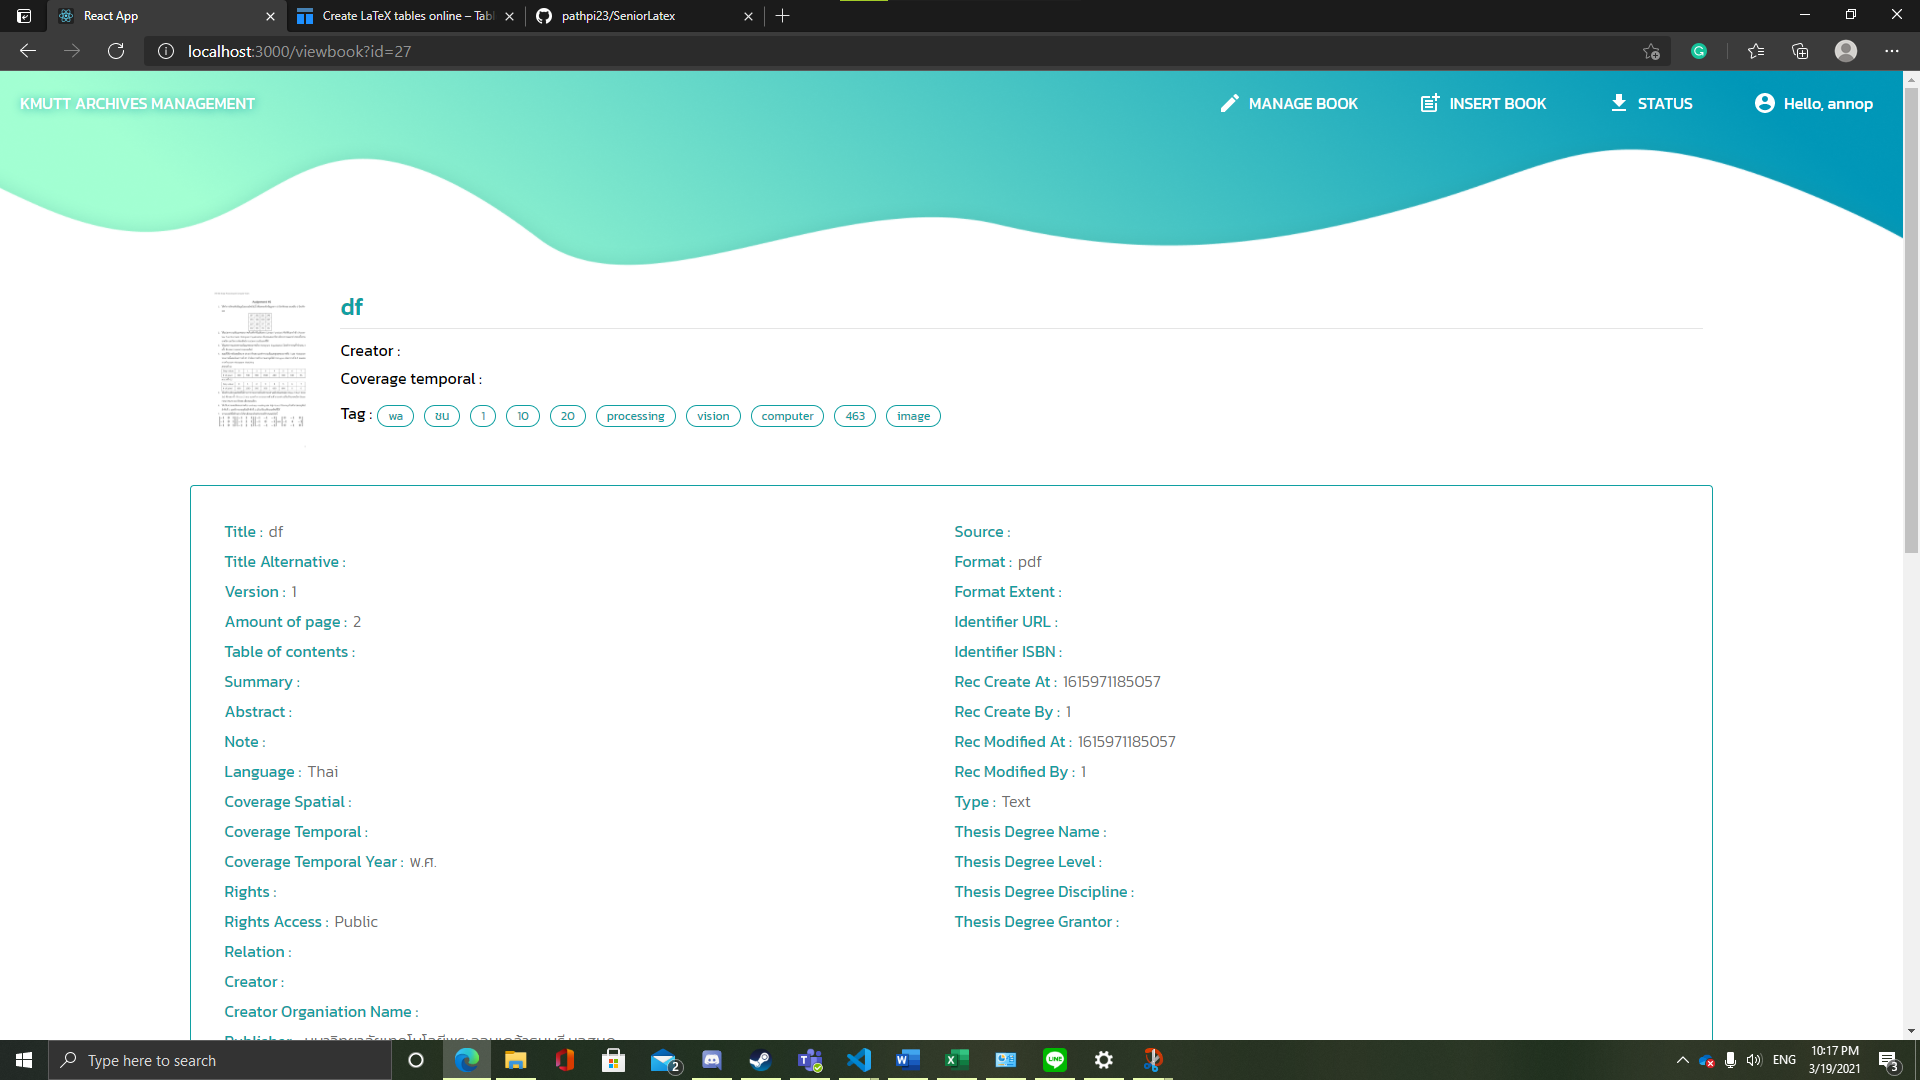
\includegraphics[scale=0.2]{webview2}
    \caption{ภาพแสดงข้อมูลของหนังสือ}\label{fig:webview2}
\end{figure}

\subsection{การแสดงการแก้ไขข้อมูลของหนังสือ}

\begin{figure}[H]
    \centering
    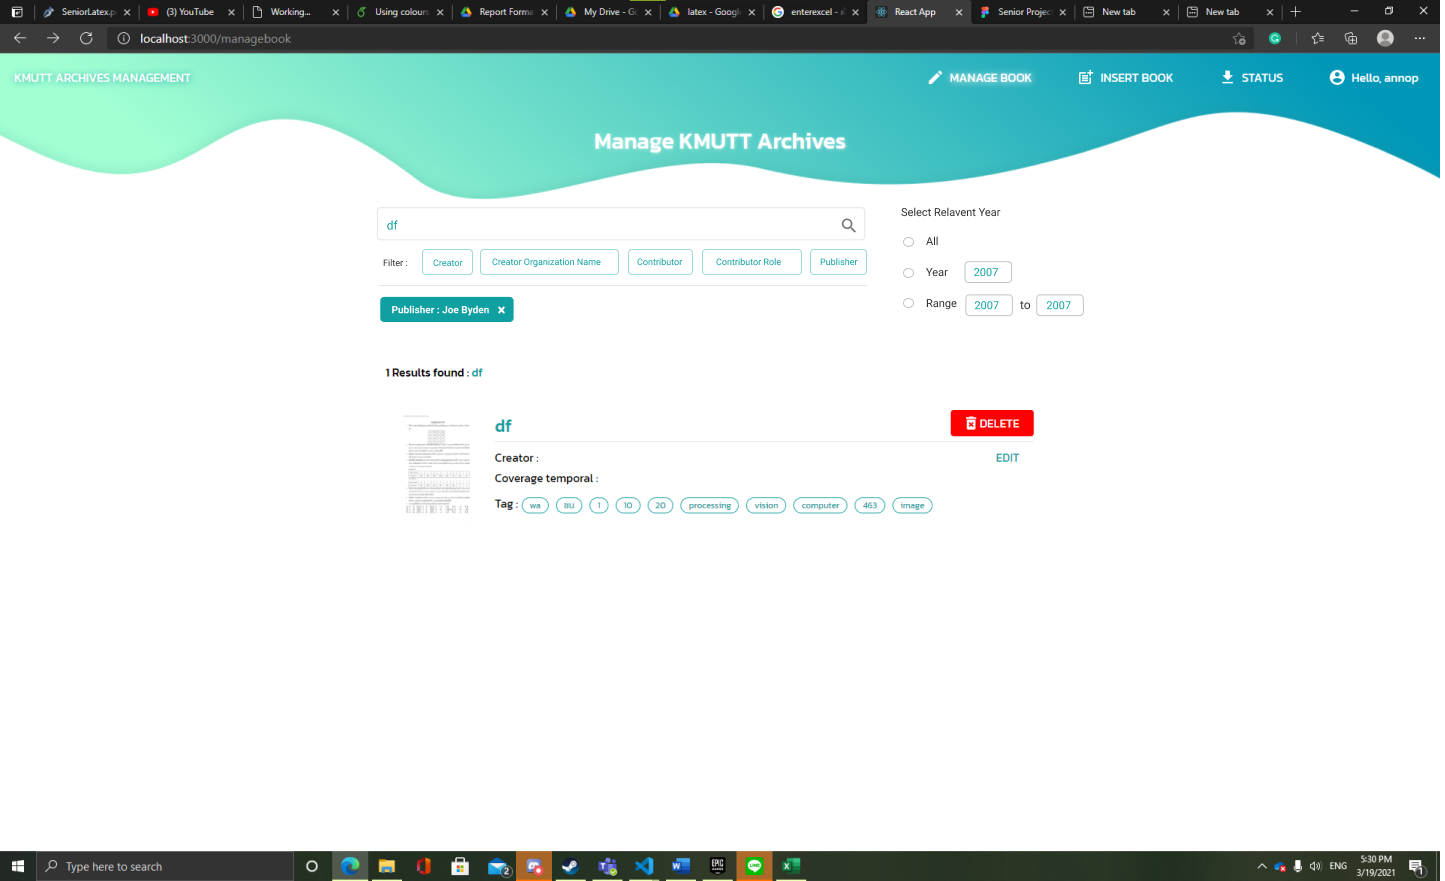
\includegraphics[scale=0.2]{webman}
    \caption{ภาพแสดงหน้าการค้นหาในหน้าการจัดการหนังสือ}\label{fig:webman}
\end{figure}

\begin{figure}[H]
    \centering
    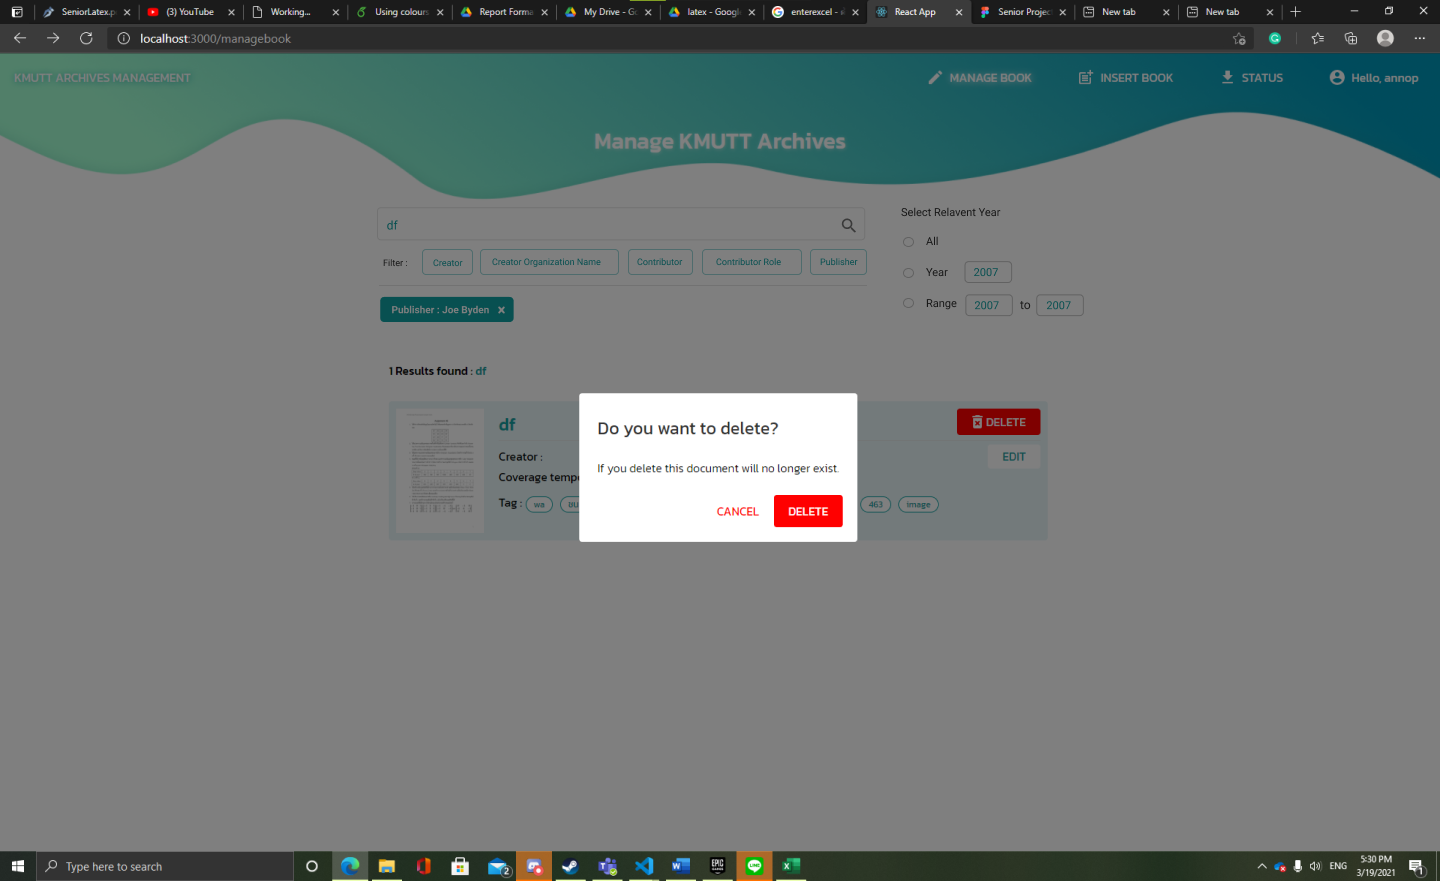
\includegraphics[scale=0.2]{webdel}
    \caption{ภาพแสดงหน้าการลบหนังสือ}\label{fig:webdel}
\end{figure}

\begin{figure}[H]
    \centering
    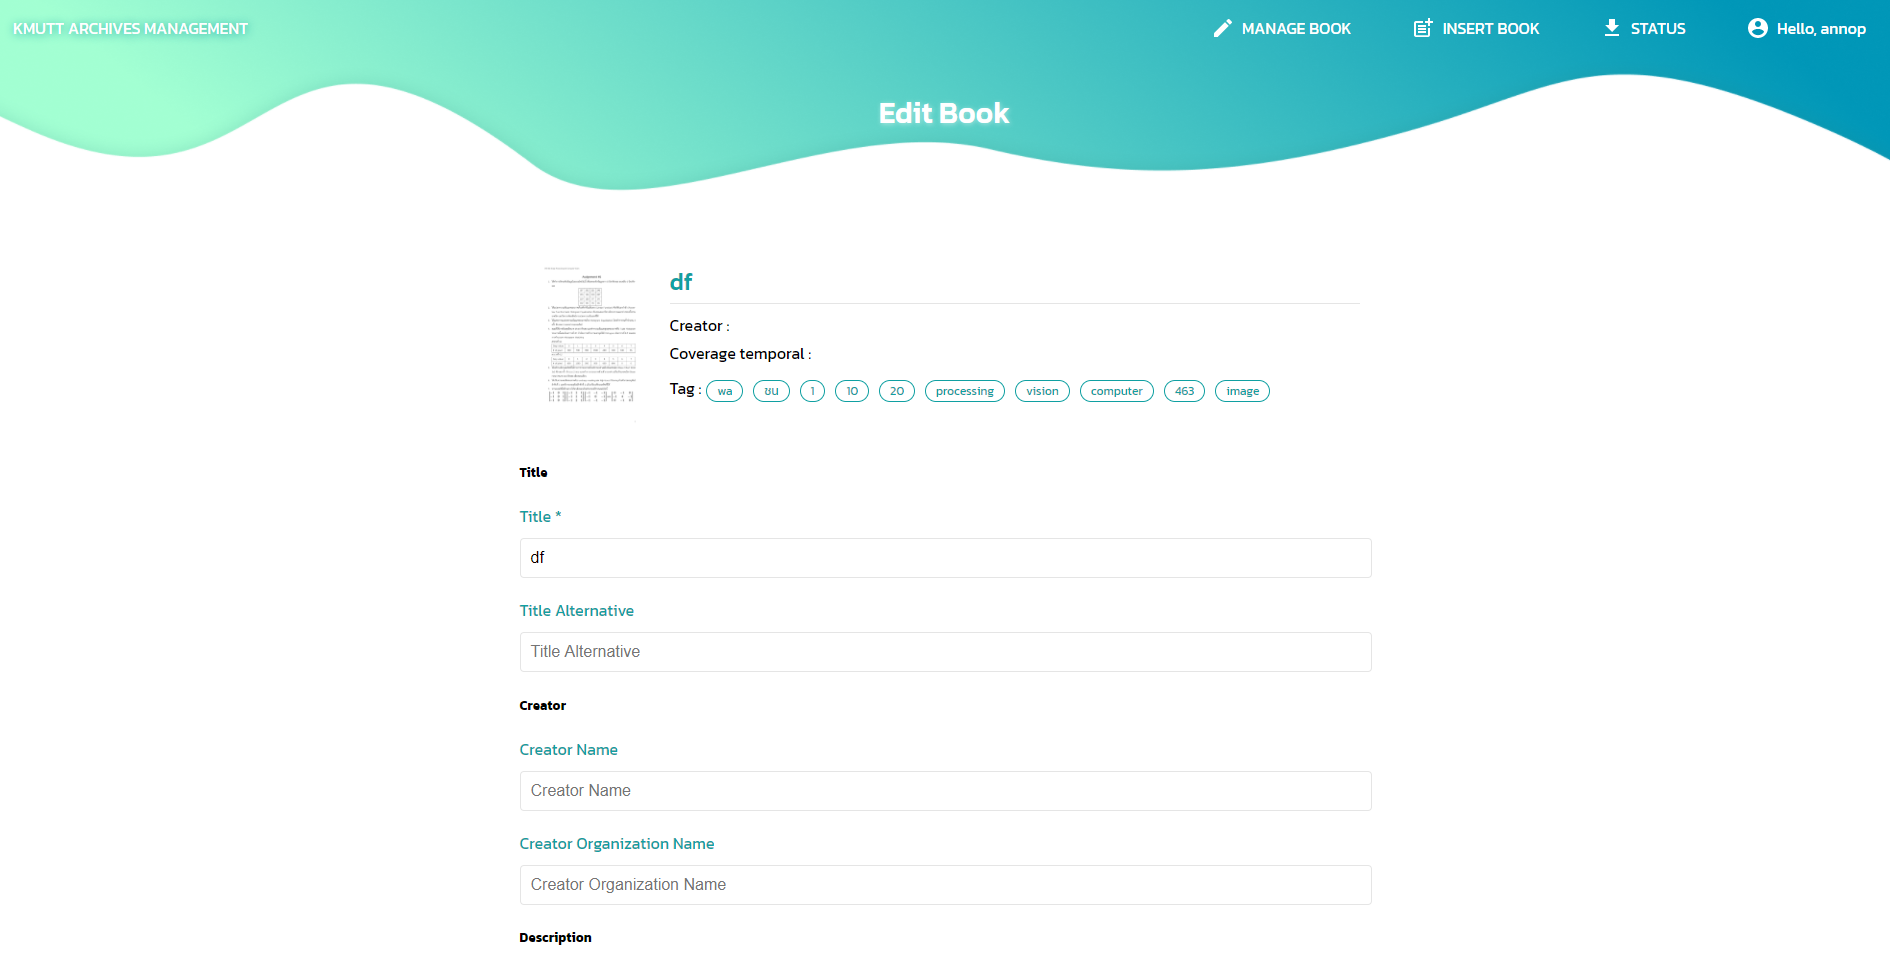
\includegraphics[scale=0.2]{webman1}
    \caption{ภาพแสดงหน้าการแก้ไขข้อมูลขั้นที่ 1}\label{fig:webman1}
\end{figure}

\begin{figure}[H]
    \centering
    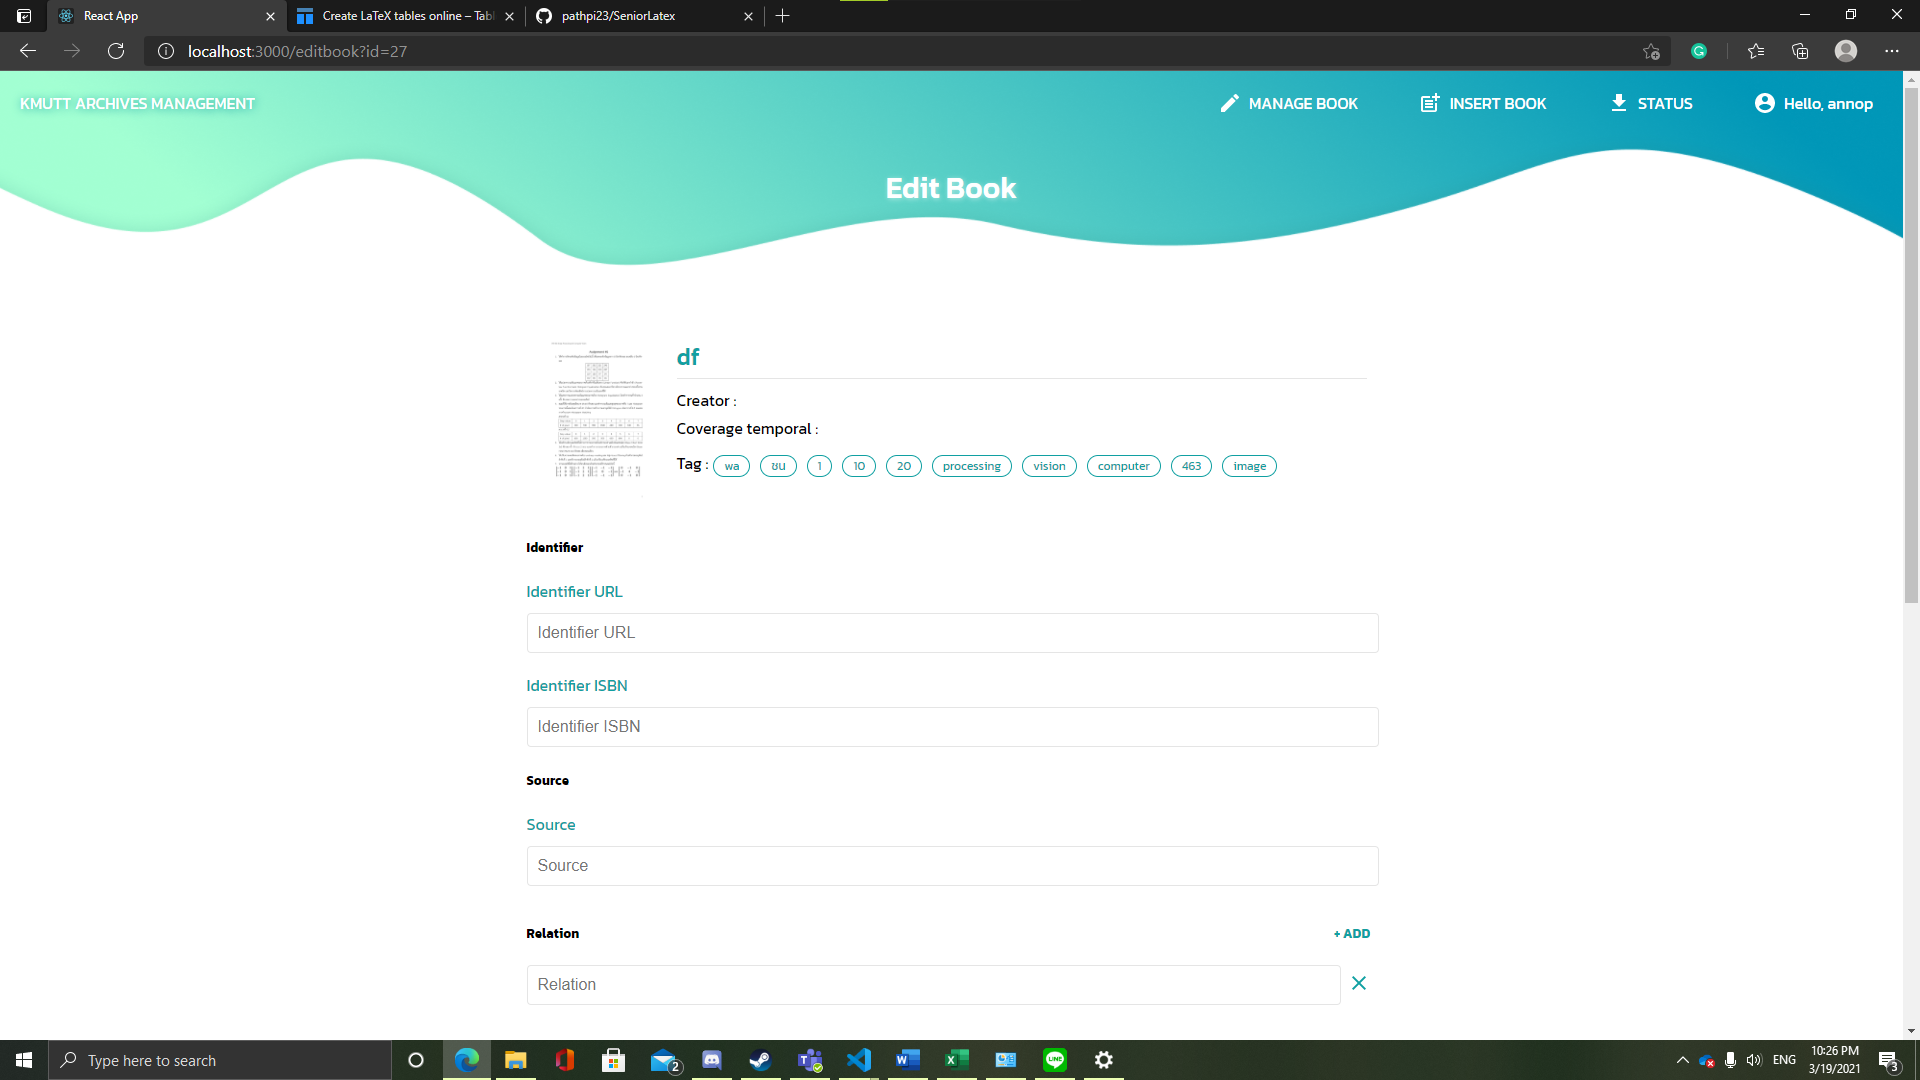
\includegraphics[scale=0.2]{webman3}
    \caption{ภาพแสดงหน้าการแก้ไขข้อมูลขั้นที่ 2}\label{fig:webman2}
\end{figure}

\begin{figure}[H]
    \centering
    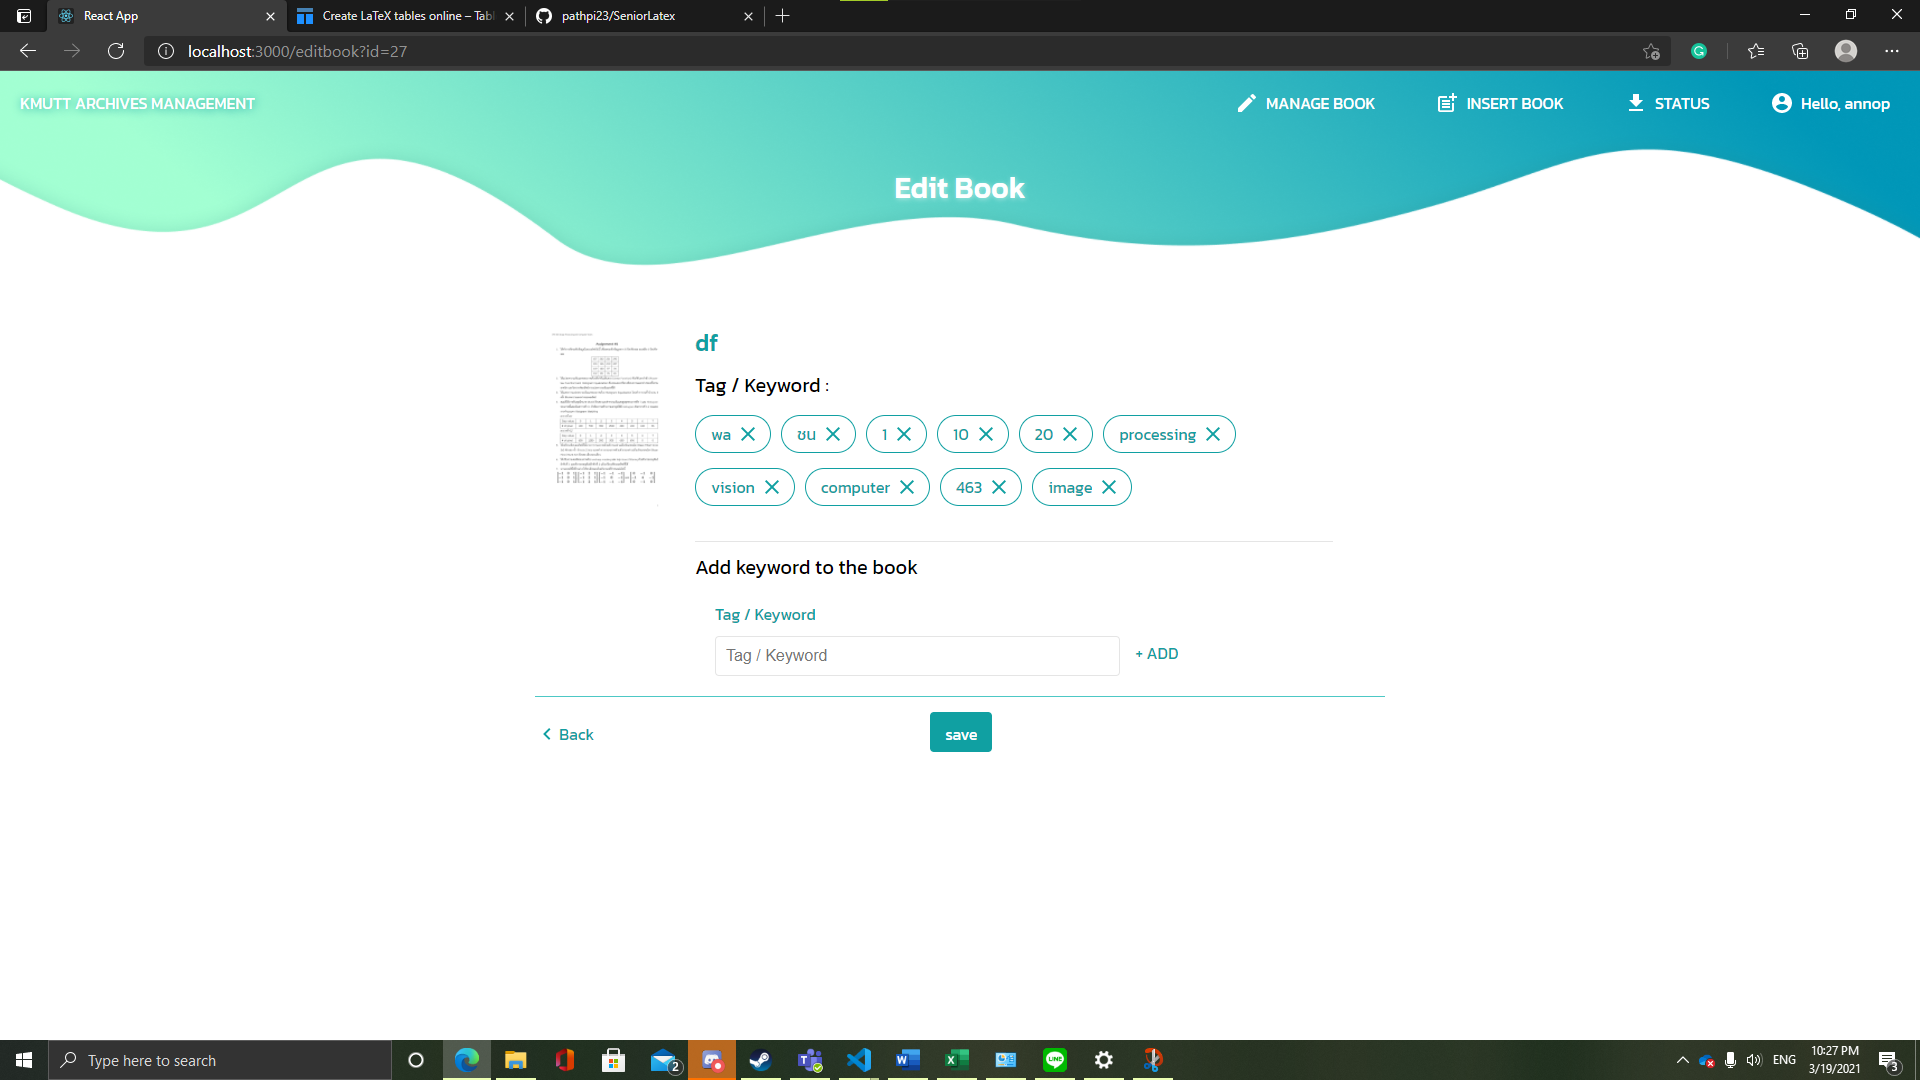
\includegraphics[scale=0.2]{webman4}
    \caption{ภาพแสดงหน้าการแก้ไขคำสำคัญ}\label{fig:webman4}
\end{figure}

การแก้ไขข้อมูลจะแก้ได้ต่อเมื่อเพิ่มข้อมูลหนังสือเสร็จสิ้นแล้วโดยที่จะสามารถแก้ไขข้อมูลในส่วนของข้อมูลหนังสือและคำสำคัญ ได้เหมือนกันกับการเพิ่มหนังสือโดยเมื่อแก้ไขเสร็จสิ้นแล้วยืนยันระบบจะทำการบันทึกข้อมูลใหม่ให้ทันที